\documentclass[12pt]{article}
\usepackage[english]{babel}
\usepackage{amsmath,amsthm}
\usepackage{amsfonts}
\usepackage{graphicx}
\newtheorem{thm}{Theorem}[section]
\newtheorem{cor}[thm]{Corollary}
\newtheorem{lem}[thm]{Lemma}
\newtheorem{prop}[thm]{Proposition}
\theoremstyle{definition}
\newtheorem{defn}[thm]{Definition}
\theoremstyle{remark}
\newtheorem{rem}[thm]{Remark}
\numberwithin{equation}{section}
\begin{document}
\title{Regression of KL Software Distribution   }
\author{KL Software Libraries}
\date{Thu Nov 15 07:31:53 2012
}
\maketitle
\textbf{ KL Libraryt unit test ouput.  This LaTex file and the associated diagrams 		are produced by the KL software libraries.}
\subsubsection{Matrix Exponential }
\begin{itemize}
\item Number or training points = 1024
\item Feature dimension = 3
\item Number or classes = 3
\end{itemize}
{The mean vectors of the 3 classes}

$\mu_1 = \left(
\begin{array}{
ccc}
+1.90000 & +0.10000 & +0.10000 \\
\end{array}
\right)$

$\mu_2 = \left(
\begin{array}{
ccc}
+0.10000 & +1.90000 & +0.10000 \\
\end{array}
\right)$

$\mu_3 = \left(
\begin{array}{
ccc}
+0.00000 & +0.00000 & +1.90000 \\
\end{array}
\right)$

A random SPD covairance matrix is generated for each of the classes.\newline

$\rho_1 = \left(
\begin{array}{
ccc}
+2.041 & +0.425 & +0.216 \\
+0.425 & +3.563 & +0.025 \\
+0.216 & +0.025 & +1.562 \\
\end{array}
\right)$

$\rho_2 = \left(
\begin{array}{
ccc}
+3.595 & +0.387 & -0.316 \\
+0.387 & +2.025 & -0.084 \\
-0.316 & -0.084 & +2.906 \\
\end{array}
\right)$

$\rho_3 = \left(
\begin{array}{
ccc}
+1.711 & -0.132 & +0.317 \\
-0.132 & +3.363 & -0.092 \\
+0.317 & -0.092 & +1.742 \\
\end{array}
\right)$

Verify $L_1$ condition number of covariance. The diagonal entries of the matrix have the form $(0.5 + U(0,1) )*dim(Dom(Cov))$
The lower-diagonal entries take the form $U(0,1) - 0.5$. 
The $L_1$ condition numbers are :
\begin{itemize}
\item +2.901
\item +2.435
\item +2.639
\end{itemize}
\includegraphics[width=10.0cm,height=10.0cm]{rv1_corr.pdf}

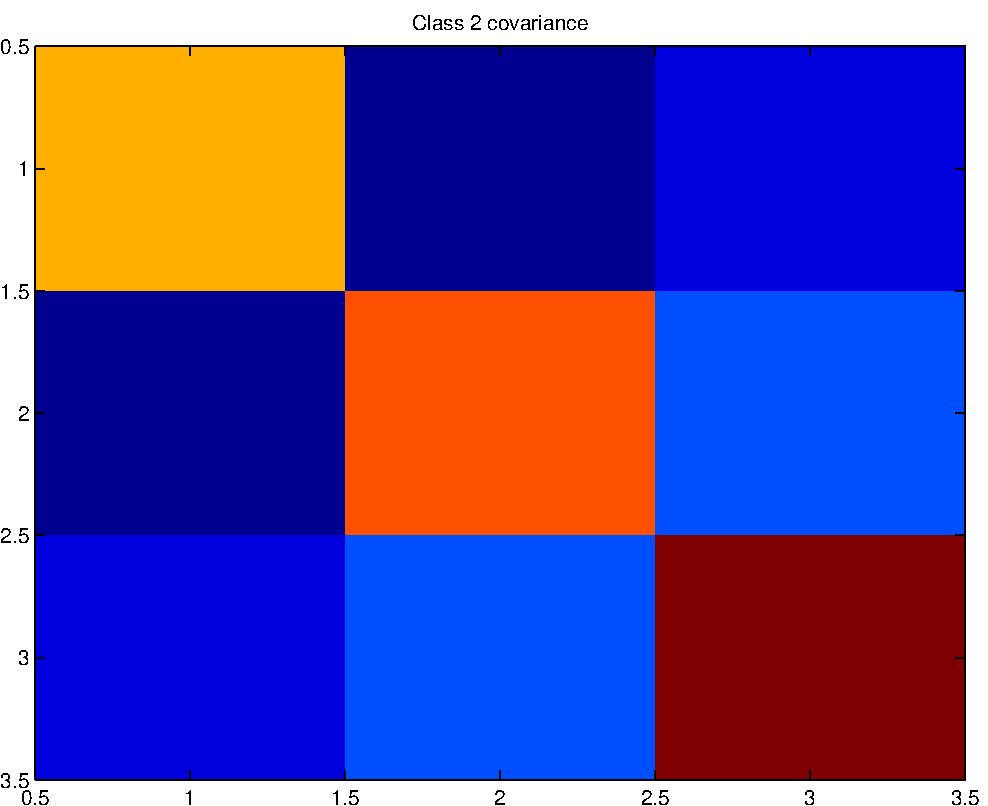
\includegraphics[width=10.0cm,height=10.0cm]{rv2_corr.pdf}

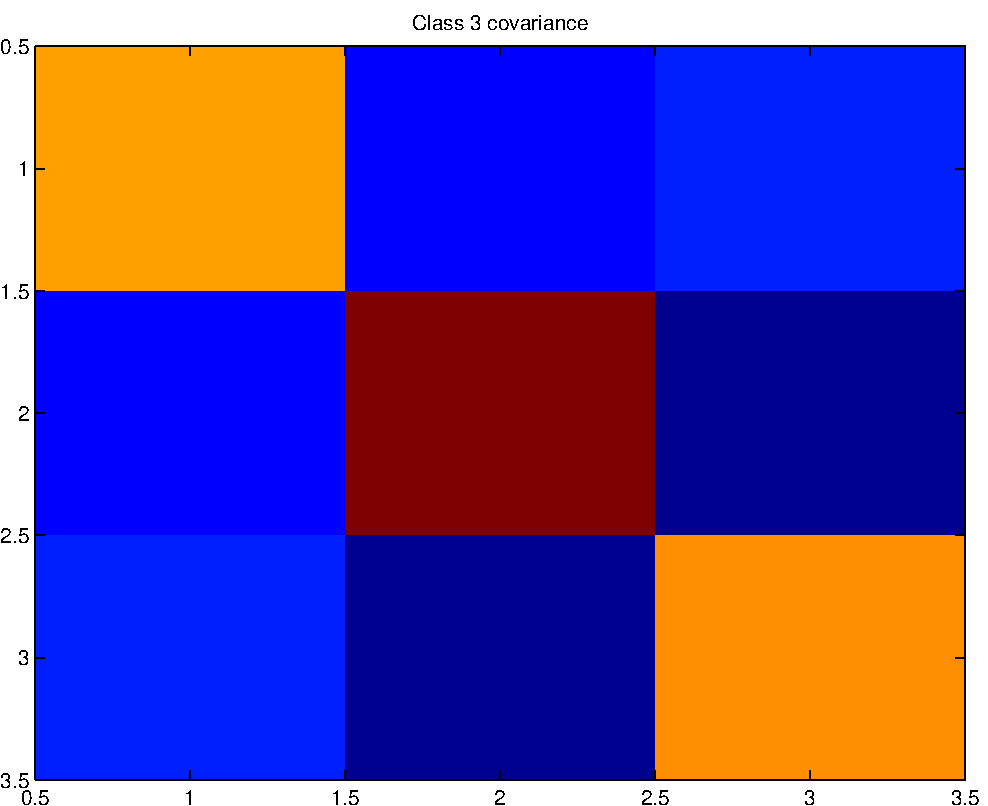
\includegraphics[width=10.0cm,height=10.0cm]{rv3_corr.pdf}

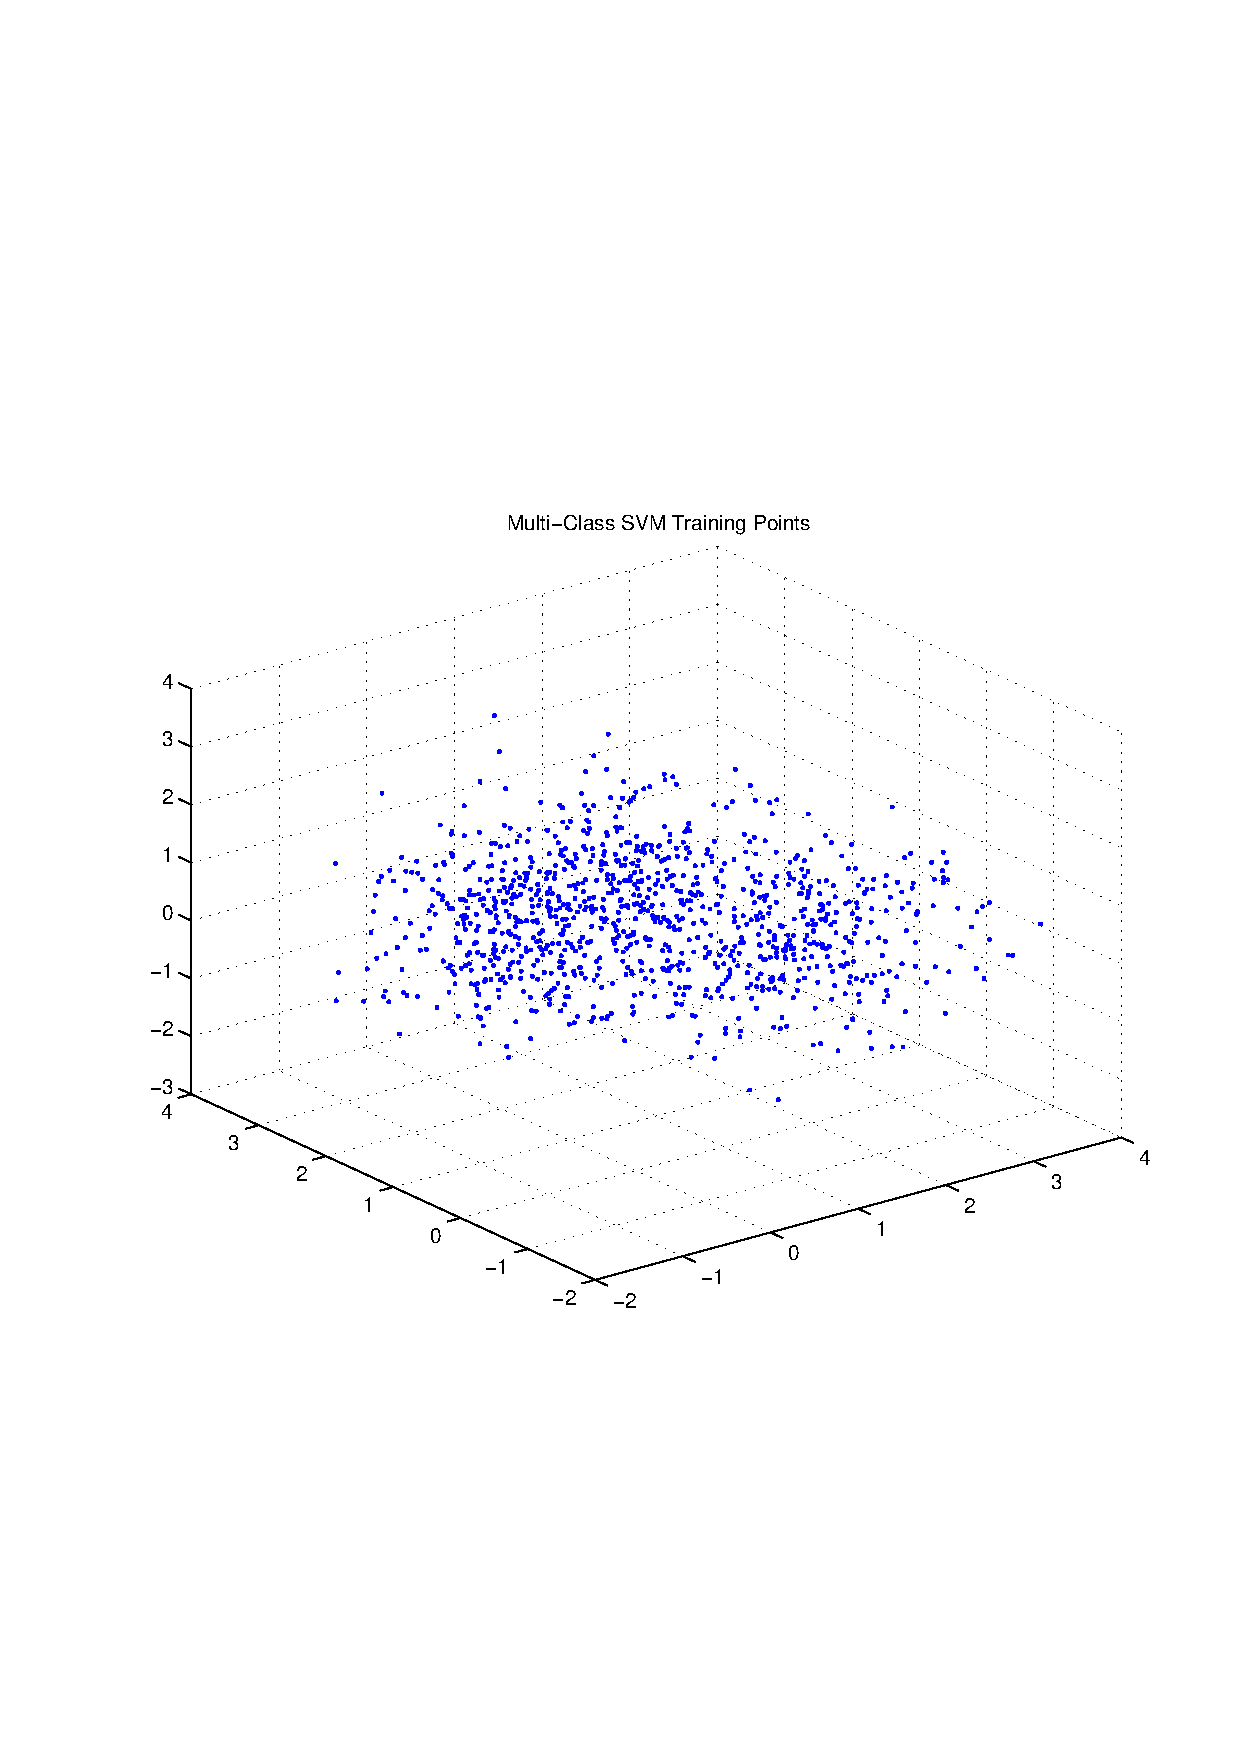
\includegraphics[width=10.0cm,height=10.0cm]{trainingPoints.pdf}

These are the SVM parameters - the RBF kernel is used\begin{itemize}
\item allOutlierFraction=0.05
\item mixingCoeff=0.3
\item smoThresh=1.0/10000.0
\item sigma=1
\end{itemize}
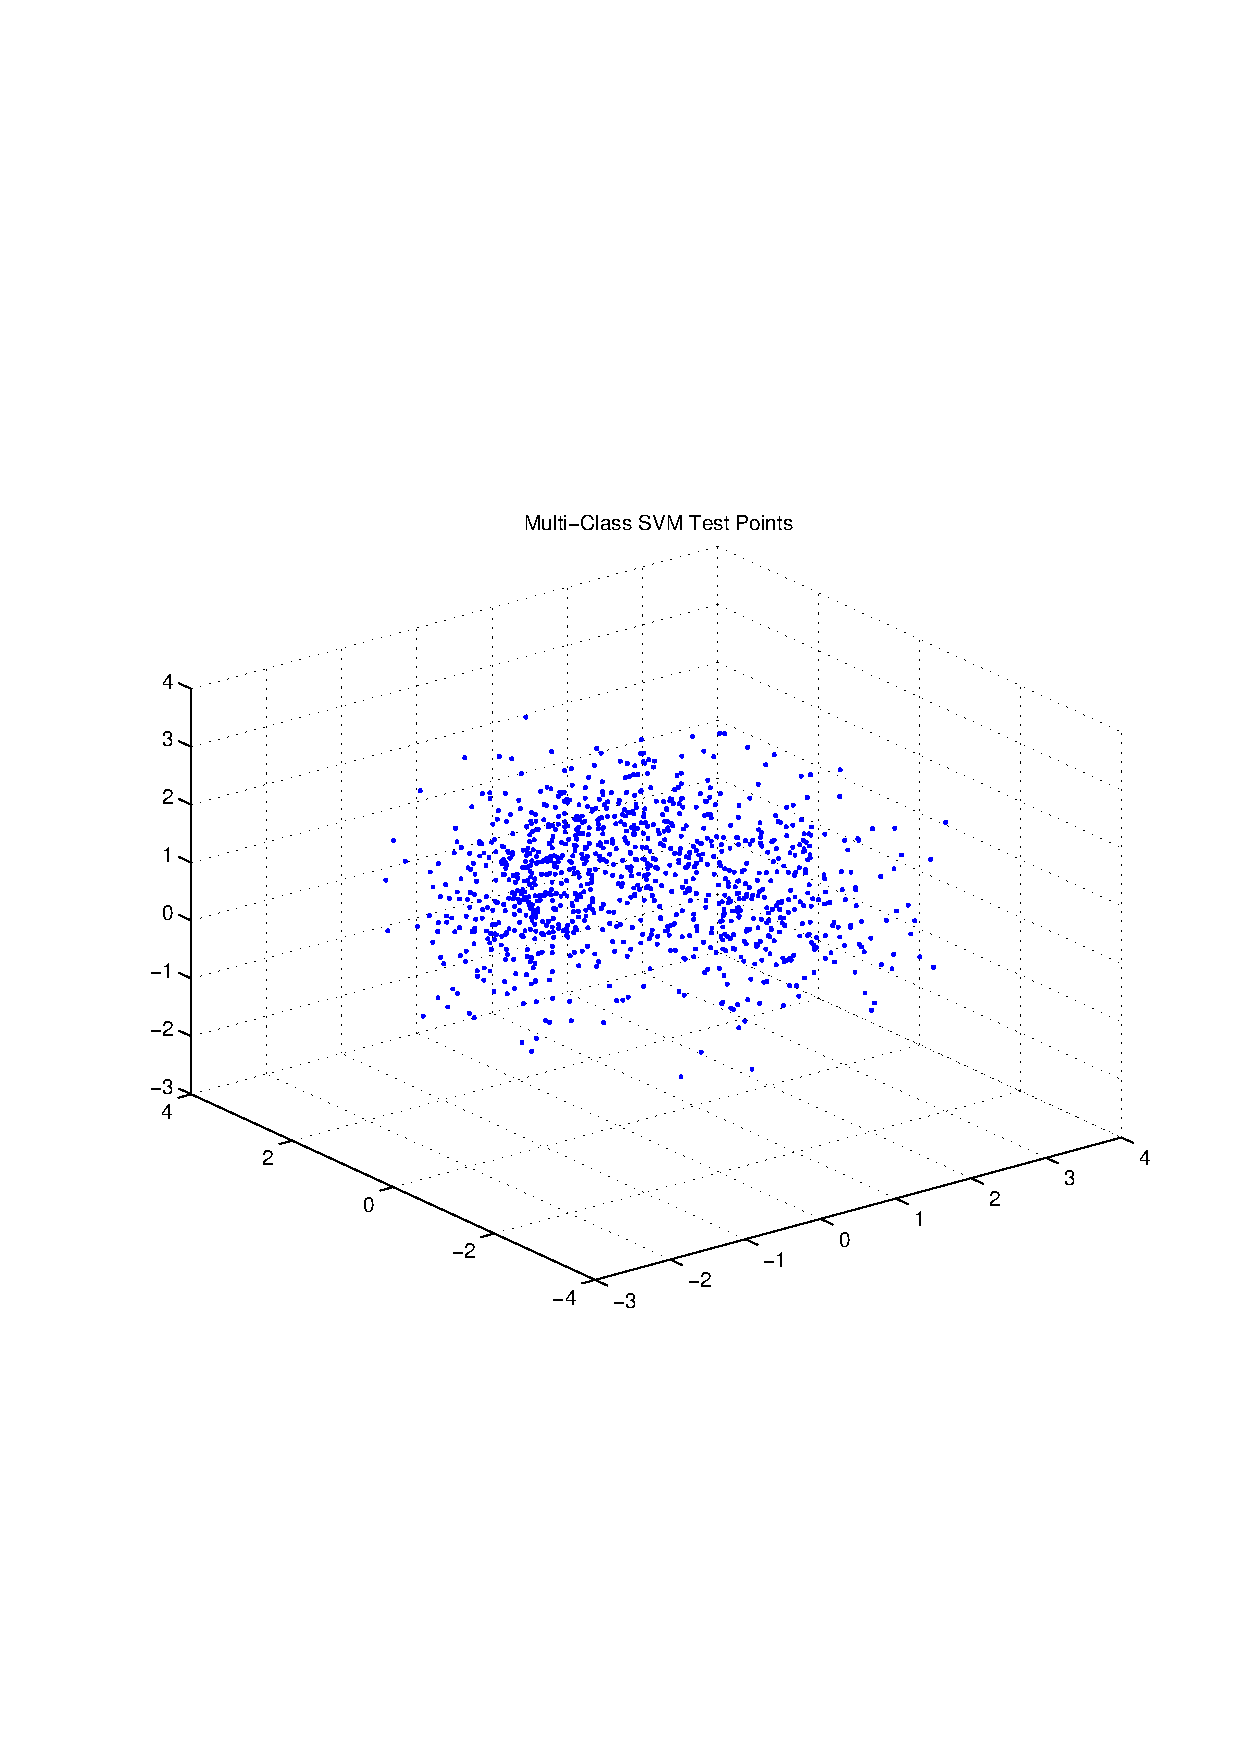
\includegraphics[width=10.0cm,height=10.0cm]{testPoints.pdf}

The marginal sample moments (mean var skew kurtosis) for training points.\newline
\begin{tabular}{ c |  c  c  c  c}
Feature & $\mu_1$ & $\mu_2$ & $\mu_3$ & $\mu_4$ \\
0 & +0.668 & +1.257 & +0.186& +2.238 \\
\hline
1 & +0.704 & +1.273 & +0.130& +2.198 \\
\hline
2 & +0.699 & +1.136 & +0.299& +2.231 \\
\hline
\end{tabular}
\newline
The marginal sample moments (mean var skew kurtosis) for test points.\newline
\begin{tabular}{ c | c  c  c  c}
Feature & $\mu_1$ & $\mu_2$ & $\mu_3$ & $\mu_4$ \\
0 & +0.677 & +1.164 & +0.344& +2.229\\
\hline
1 & +0.668 & +1.276 & +0.170& +2.180\\
\hline
2 & +0.717 & +1.083 & +0.271& +2.195\\
\hline
\end{tabular}\newline
\includegraphics[width=10.0cm,height=10.0cm]{classDiffs.pdf}

The error rate for this run is +0.044\newline
QueryPerformanceCounter  =  +20.445
\subsubsection{Multiclass Support Vector Machine }
\begin{itemize}
\item Number or training points = 1024
\item Feature dimension = 3
\item Number or classes = 3
\end{itemize}
{The mean vectors of the 3 classes}

$\mu_1 = \left(
\begin{array}{
ccc}
+1.90000 & +0.10000 & +0.10000 \\
\end{array}
\right)$

$\mu_2 = \left(
\begin{array}{
ccc}
+0.10000 & +1.90000 & +0.10000 \\
\end{array}
\right)$

$\mu_3 = \left(
\begin{array}{
ccc}
+0.00000 & +0.00000 & +1.90000 \\
\end{array}
\right)$

A random SPD covairance matrix is generated for each of the classes.\newline

$\rho_1 = \left(
\begin{array}{
ccc}
+2.533 & -0.193 & +0.112 \\
-0.193 & +1.541 & +0.275 \\
+0.112 & +0.275 & +3.030 \\
\end{array}
\right)$

$\rho_2 = \left(
\begin{array}{
ccc}
+1.543 & -0.012 & +0.341 \\
-0.012 & +4.348 & -0.401 \\
+0.341 & -0.401 & +1.946 \\
\end{array}
\right)$

$\rho_3 = \left(
\begin{array}{
ccc}
+2.334 & +0.208 & +0.246 \\
+0.208 & +3.514 & -0.080 \\
+0.246 & -0.080 & +4.130 \\
\end{array}
\right)$

Verify $L_1$ condition number of covariance. The diagonal entries of the matrix have the form $(0.5 + U(0,1) )*dim(Dom(Cov))$
The lower-diagonal entries take the form $U(0,1) - 0.5$. 
The $L_1$ condition numbers are :
\begin{itemize}
\item +2.675
\item +3.828
\item +2.167
\end{itemize}
\includegraphics[width=10.0cm,height=10.0cm]{rv1_corr.pdf}

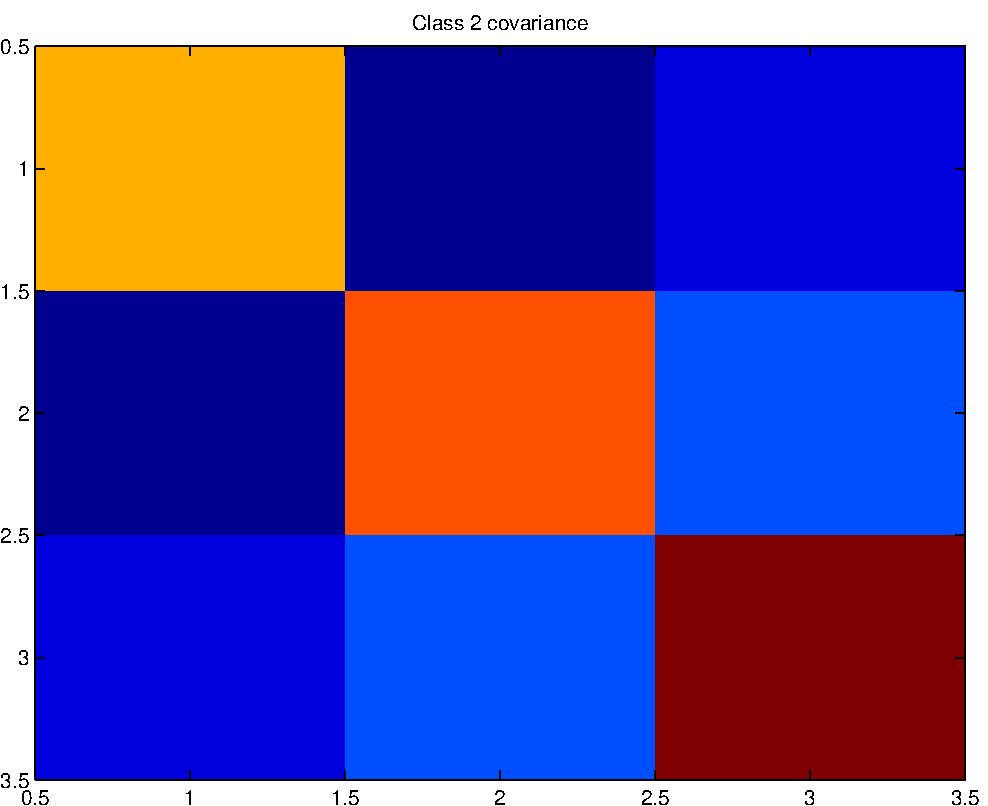
\includegraphics[width=10.0cm,height=10.0cm]{rv2_corr.pdf}

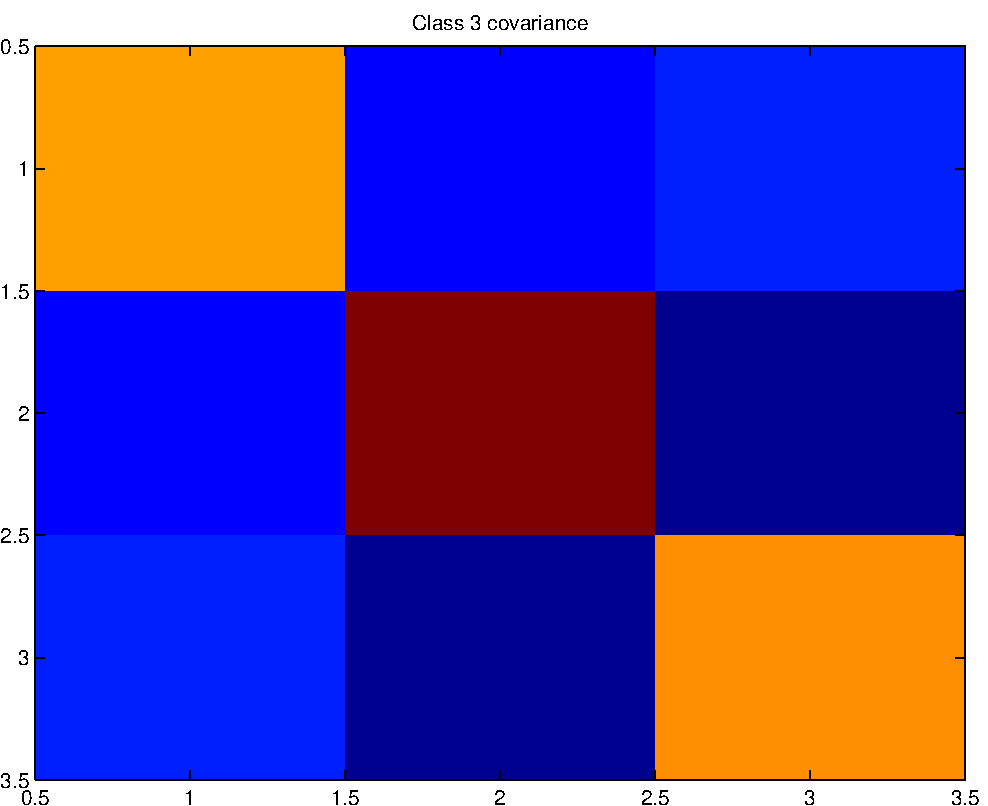
\includegraphics[width=10.0cm,height=10.0cm]{rv3_corr.pdf}

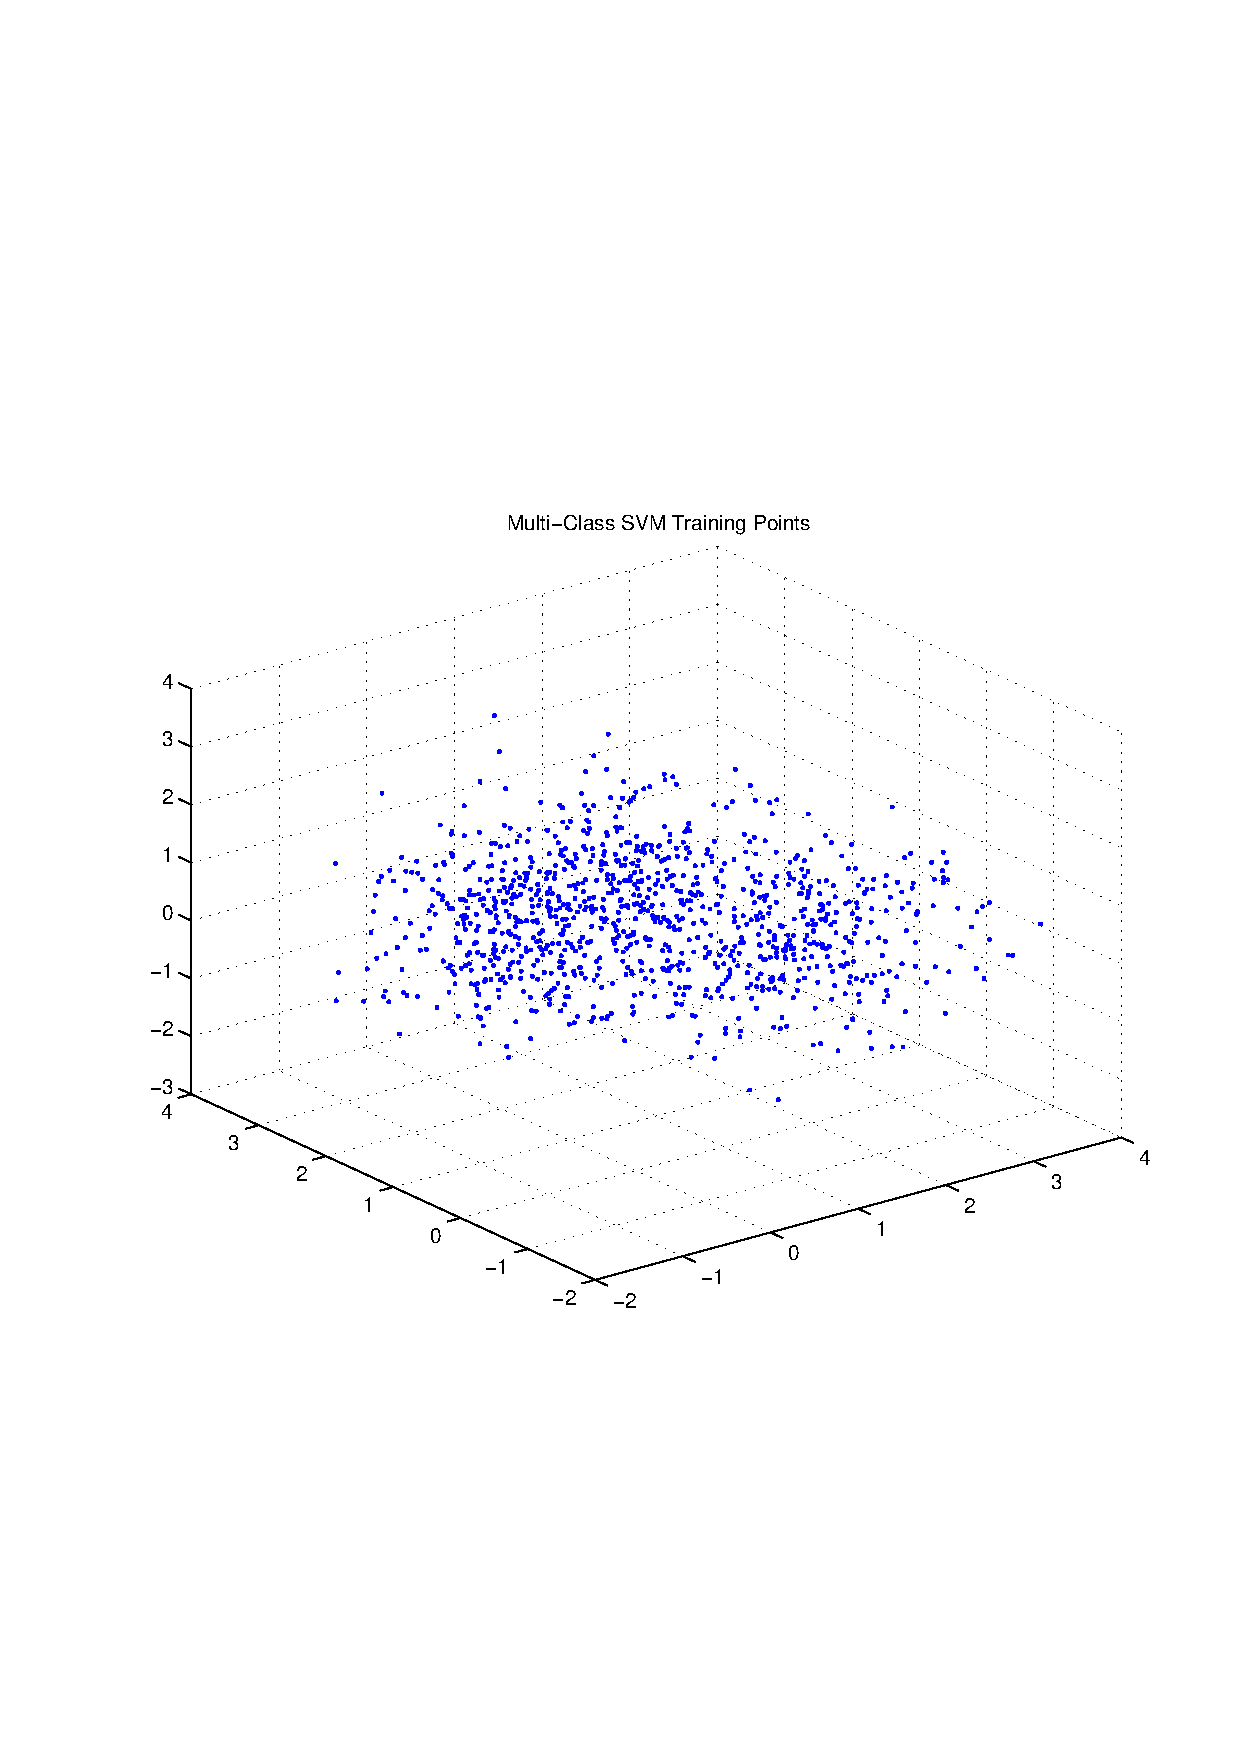
\includegraphics[width=10.0cm,height=10.0cm]{trainingPoints.pdf}

These are the SVM parameters - the RBF kernel is used\begin{itemize}
\item allOutlierFraction=0.05
\item mixingCoeff=0.3
\item smoThresh=1.0/10000.0
\item sigma=1
\end{itemize}
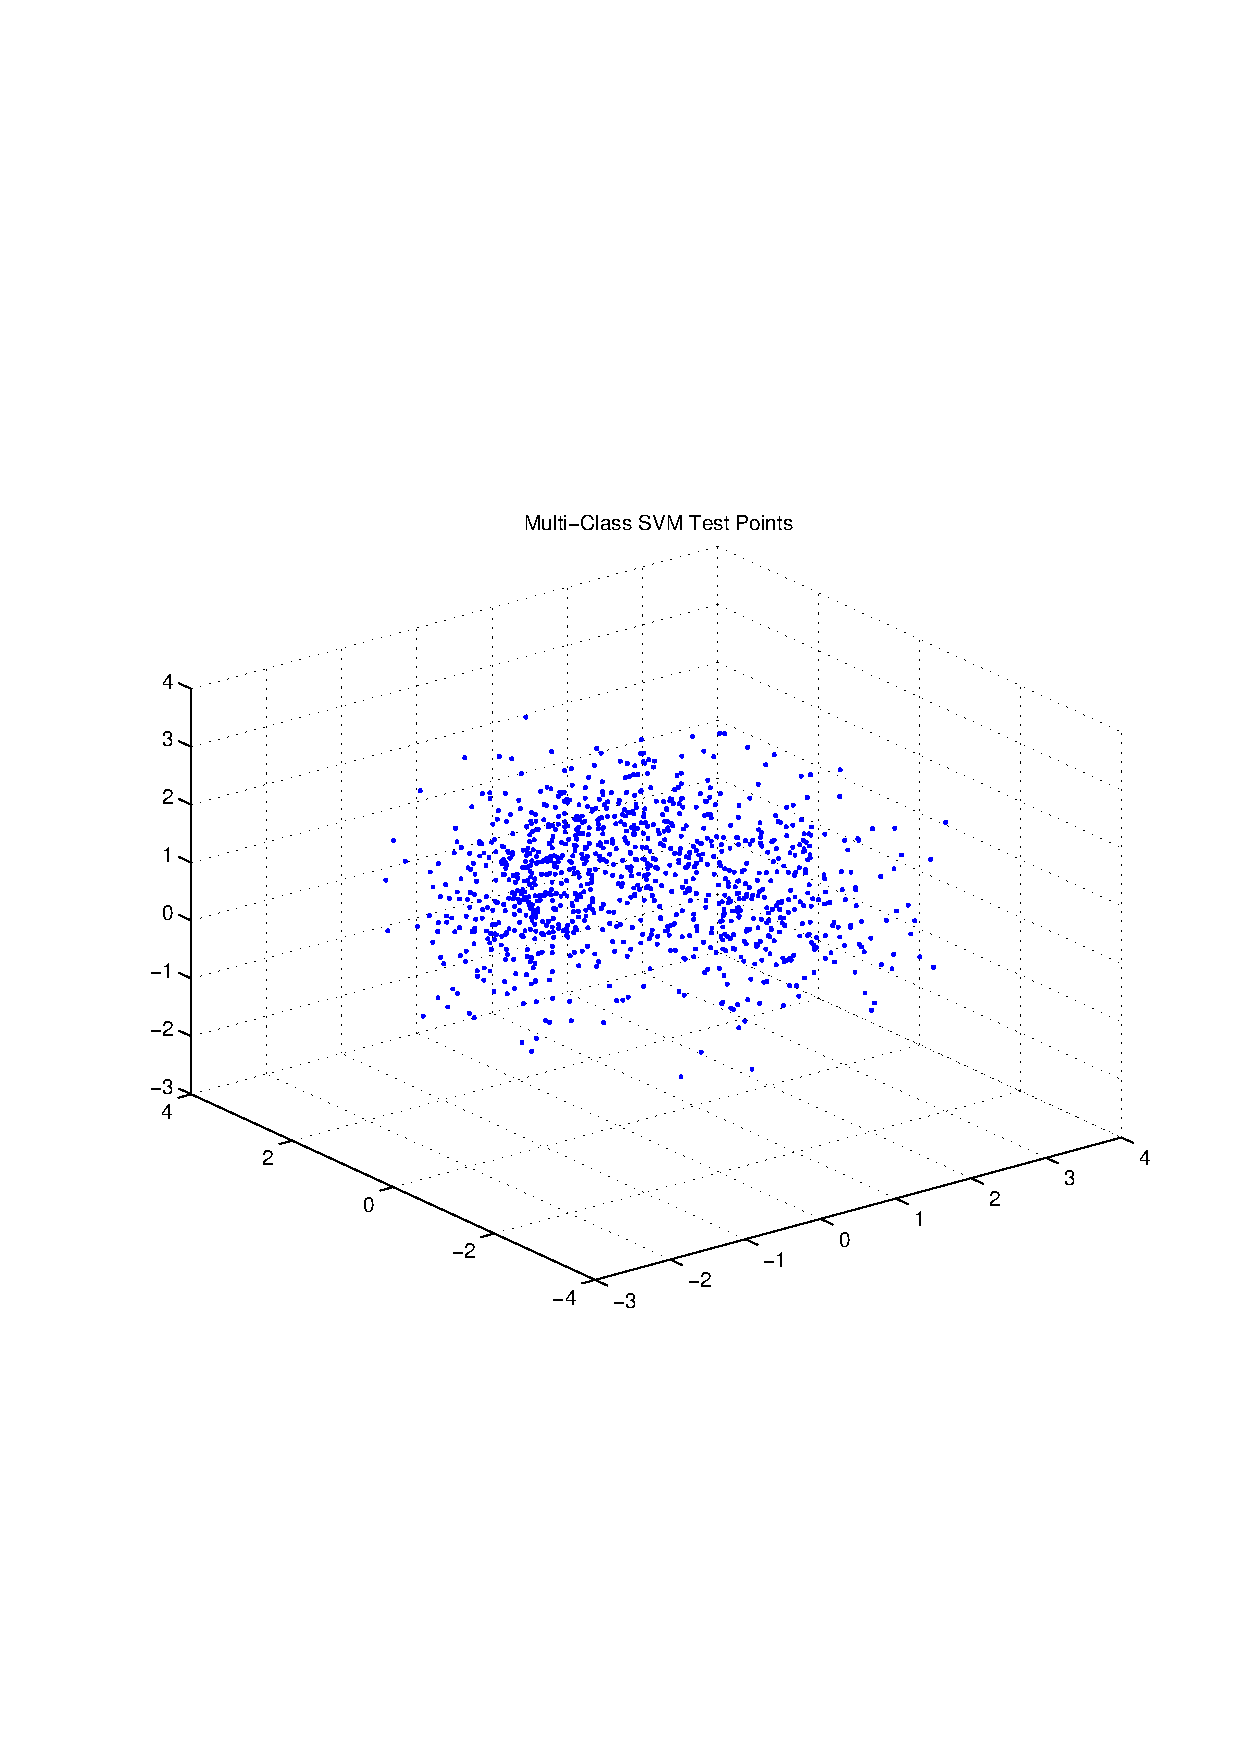
\includegraphics[width=10.0cm,height=10.0cm]{testPoints.pdf}

The marginal sample moments (mean var skew kurtosis) for training points.\newline
\begin{tabular}{ c |  c  c  c  c}
Feature & $\mu_1$ & $\mu_2$ & $\mu_3$ & $\mu_4$ \\
0 & +0.670 & +1.190 & +0.398& +2.330 \\
\hline
1 & +0.705 & +1.315 & +0.569& +2.734 \\
\hline
2 & +0.706 & +1.329 & +0.552& +2.757 \\
\hline
\end{tabular}
\newline
The marginal sample moments (mean var skew kurtosis) for test points.\newline
\begin{tabular}{ c | c  c  c  c}
Feature & $\mu_1$ & $\mu_2$ & $\mu_3$ & $\mu_4$ \\
0 & +0.676 & +1.127 & +0.516& +2.456\\
\hline
1 & +0.674 & +1.302 & +0.600& +2.735\\
\hline
2 & +0.722 & +1.247 & +0.537& +2.639\\
\hline
\end{tabular}\newline
\includegraphics[width=10.0cm,height=10.0cm]{classDiffs.pdf}

The error rate for this run is +0.173\newline
QueryPerformanceCounter  =  +6.836
\subsubsection{Random Number Generator }
The sample size generated for this run is 100000.

\newpage
uniform \begin{tabular}{|c|c|c|c|}  mean & variance & skewness & kurtosis \\  \hline
$\mu_1 = +0.500$ & $\mu_2 = +0.084$ & $\mu_3 = +0.003$ & $\mu_4 =+1.801$ \\
\end{tabular}

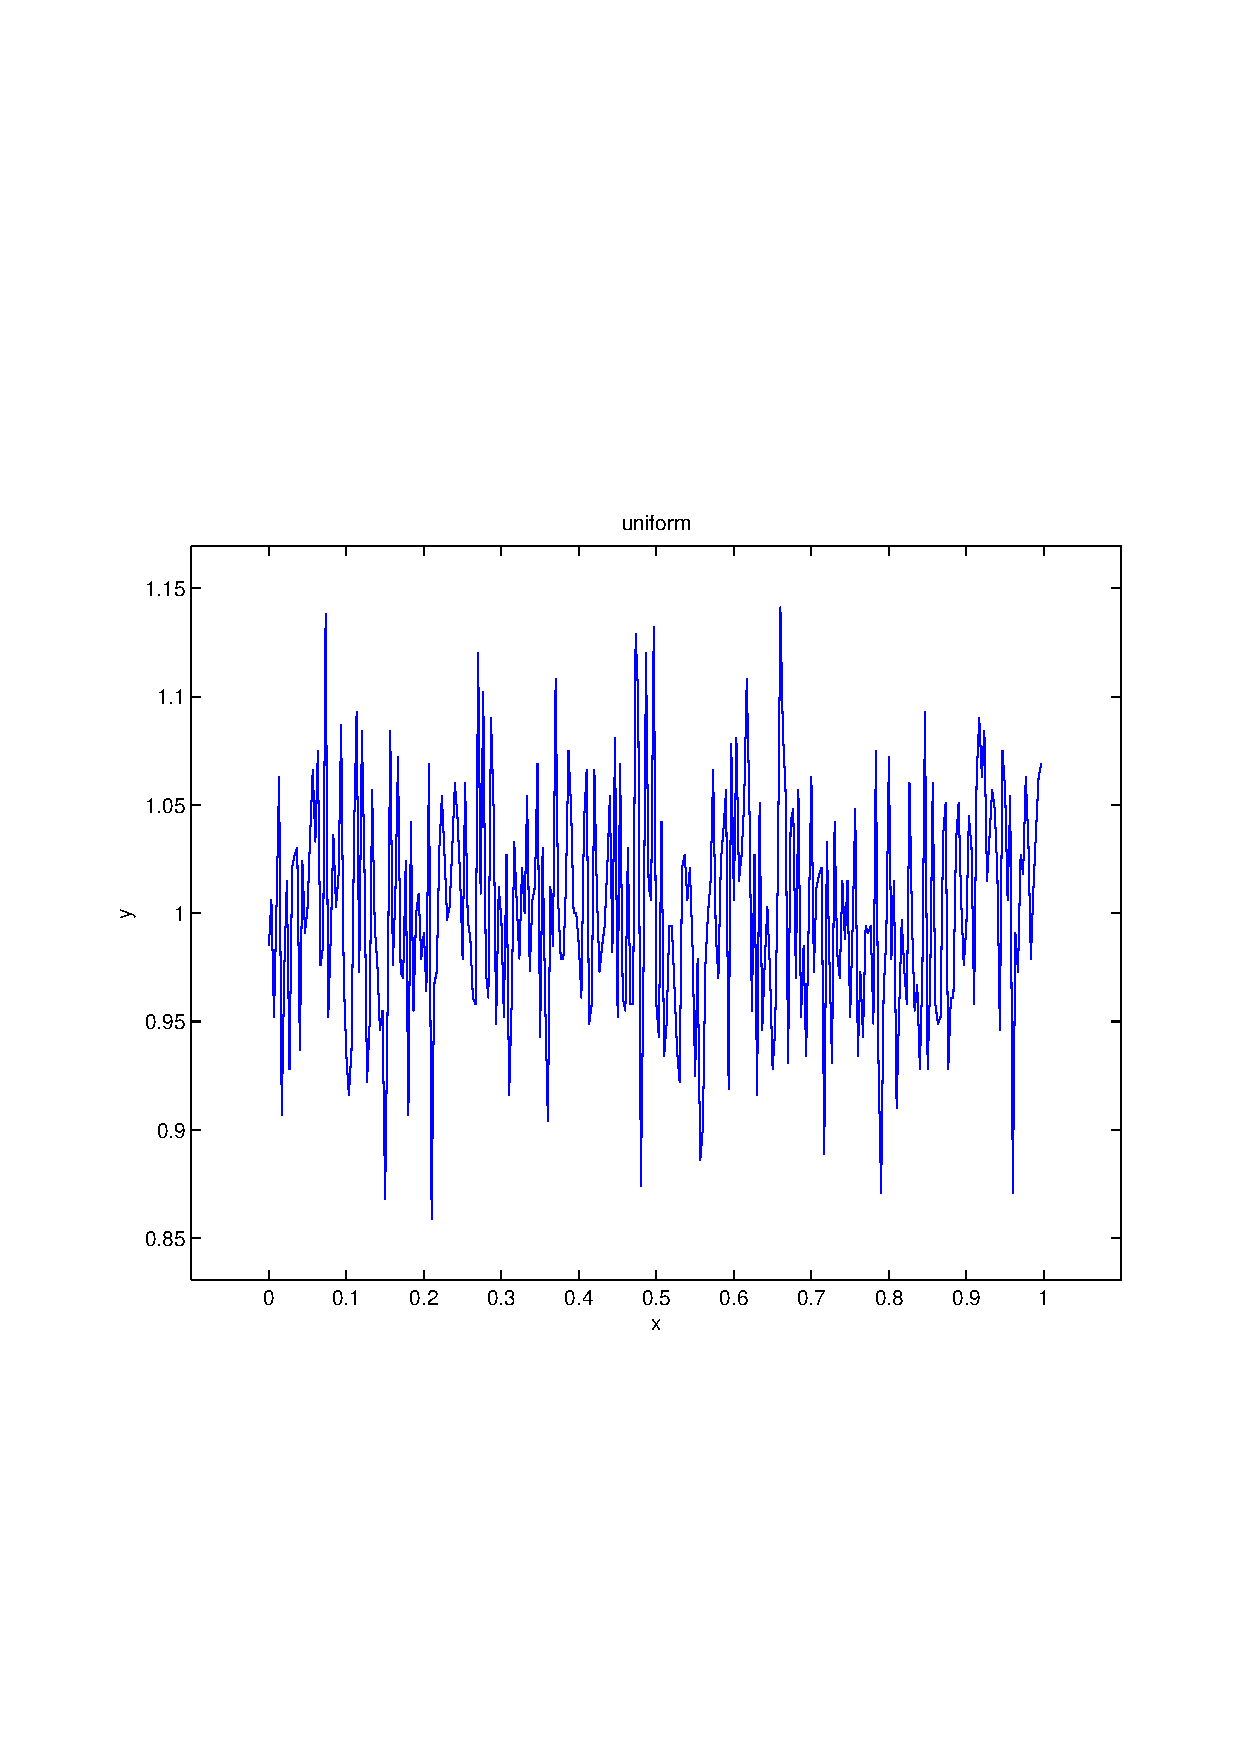
\includegraphics[width=5cm,height=5cm]{uniform.pdf}

cauchy \begin{tabular}{|c|c|c|c|}  mean & variance & skewness & kurtosis \\  \hline
$\mu_1 = +0.443$ & $\mu_2 = +0.053$ & $\mu_3 = +0.639$ & $\mu_4 =+3.281$ \\
\end{tabular}

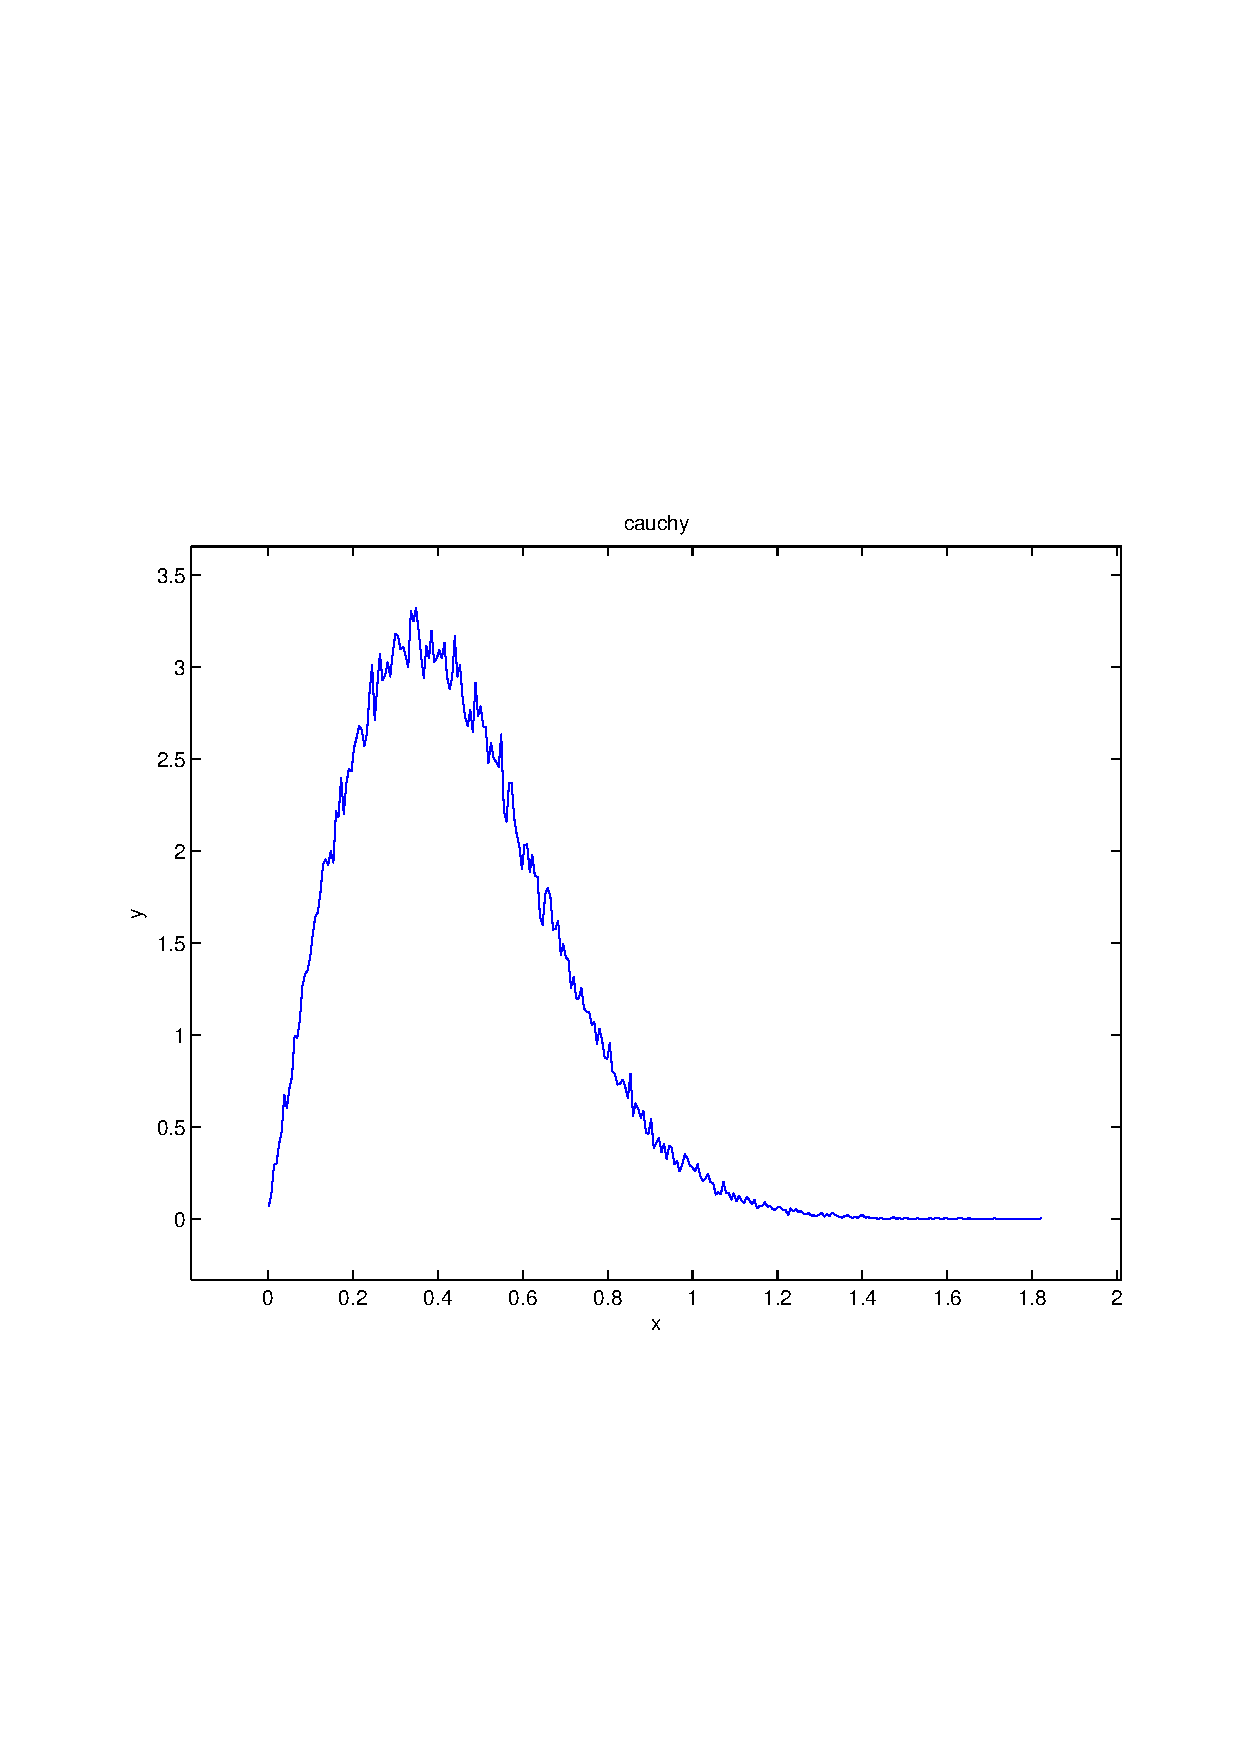
\includegraphics[width=5cm,height=5cm]{cauchy.pdf}

exponential \begin{tabular}{|c|c|c|c|}  mean & variance & skewness & kurtosis \\  \hline
$\mu_1 = +1.996$ & $\mu_2 = +3.993$ & $\mu_3 = +2.031$ & $\mu_4 =+9.308$ \\
\end{tabular}

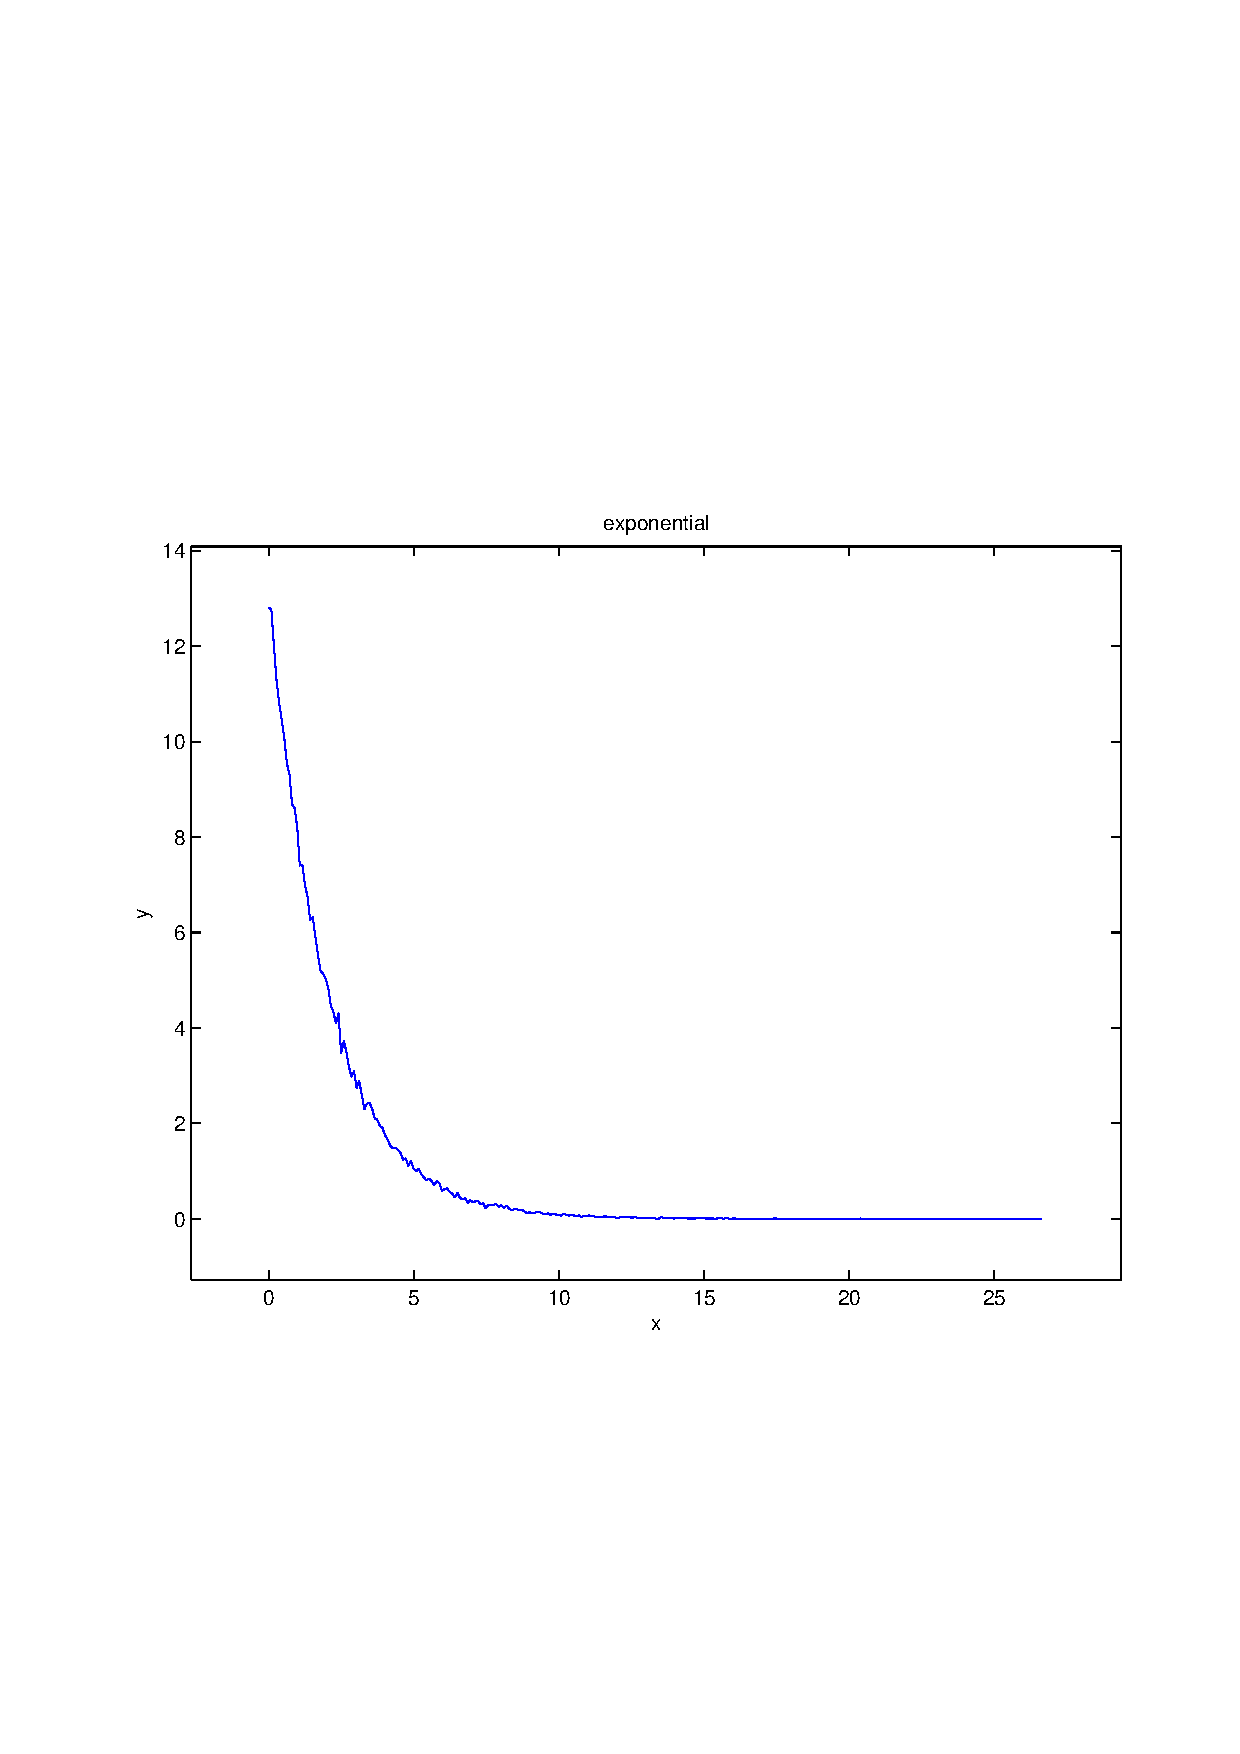
\includegraphics[width=5cm,height=5cm]{exponential.pdf}

\newpage
gamma \begin{tabular}{|c|c|c|c|}  mean & variance & skewness & kurtosis \\  \hline
$\mu_1 = +1.898$ & $\mu_2 = +1.902$ & $\mu_3 = +1.433$ & $\mu_4 =+5.995$ \\
\end{tabular}

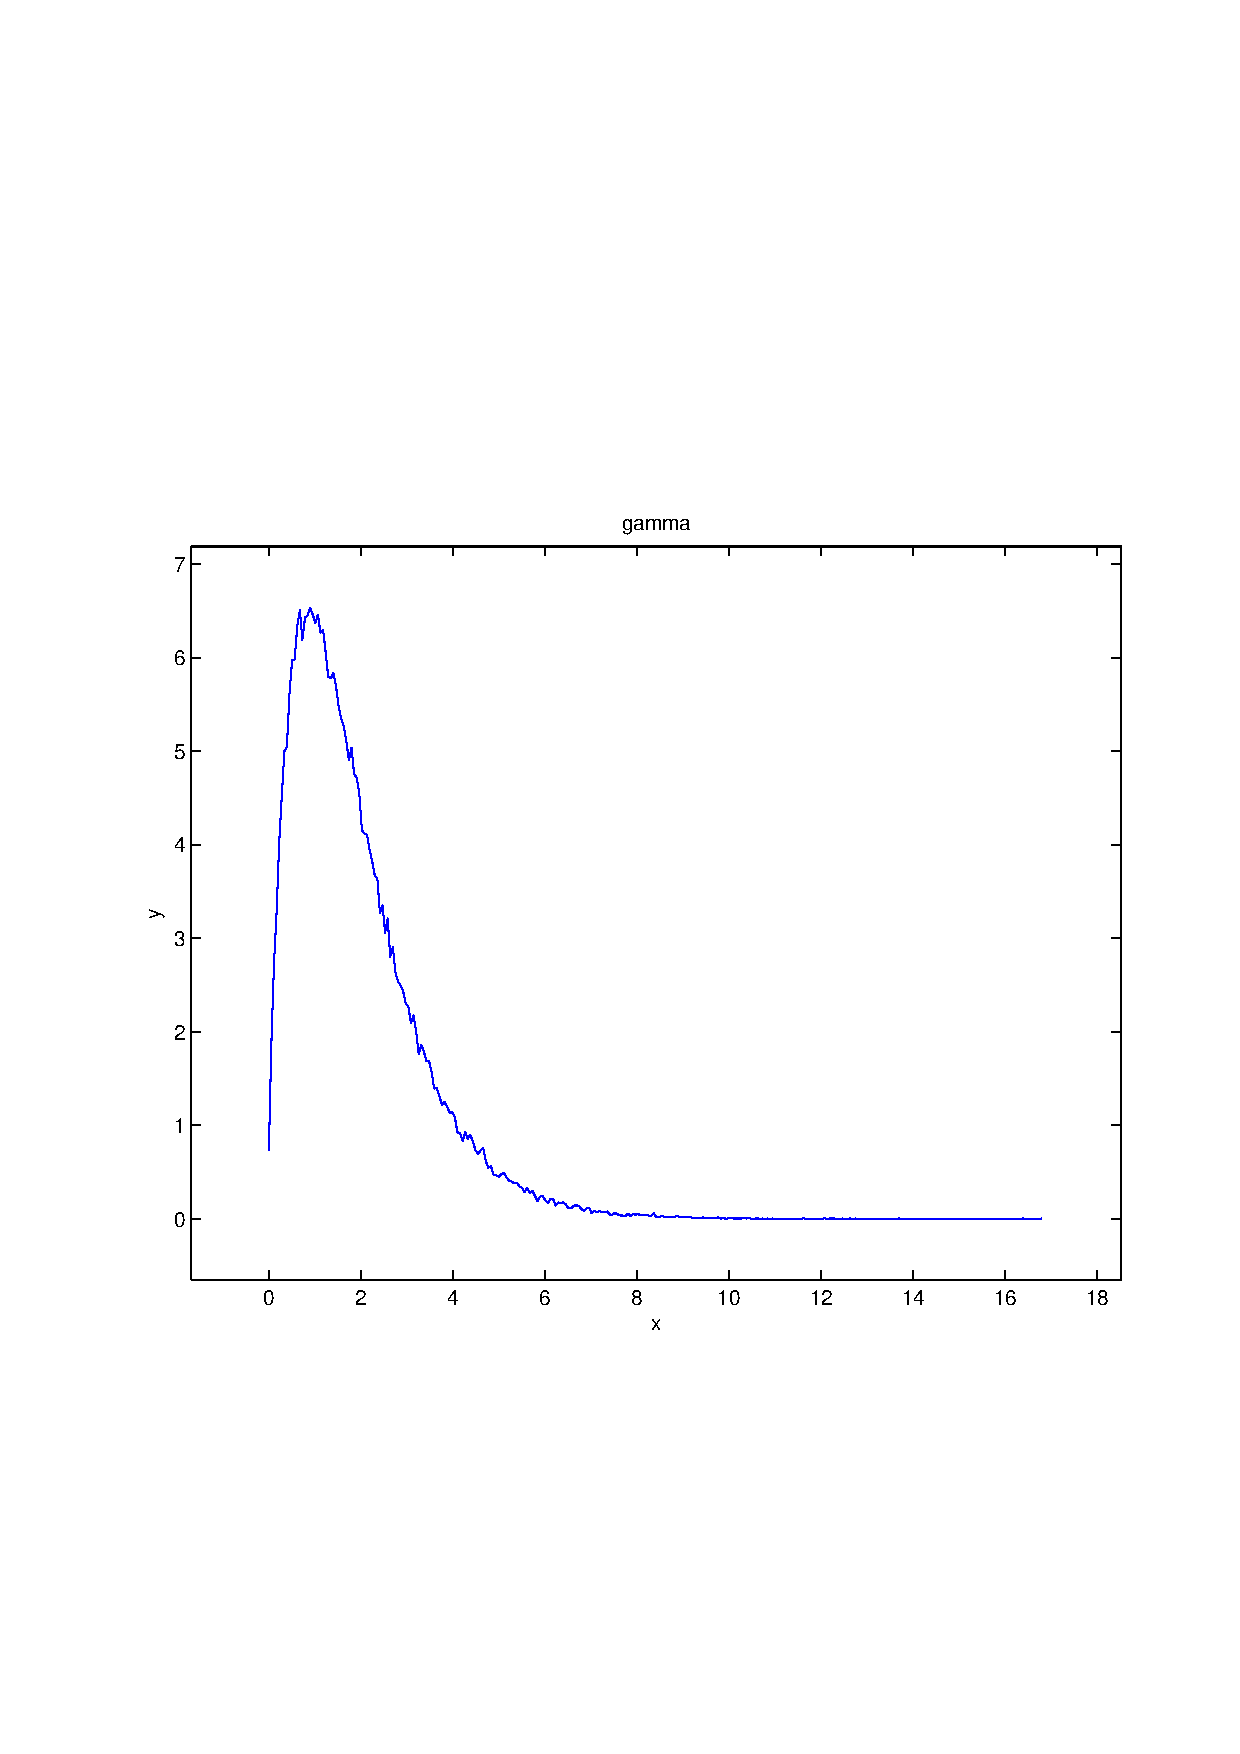
\includegraphics[width=5cm,height=5cm]{gamma.pdf}

GIG \begin{tabular}{|c|c|c|c|}  mean & variance & skewness & kurtosis \\  \hline
$\mu_1 = +0.816$ & $\mu_2 = +11.971$ & $\mu_3 = +14.941$ & $\mu_4 =+297.475$ \\
\end{tabular}

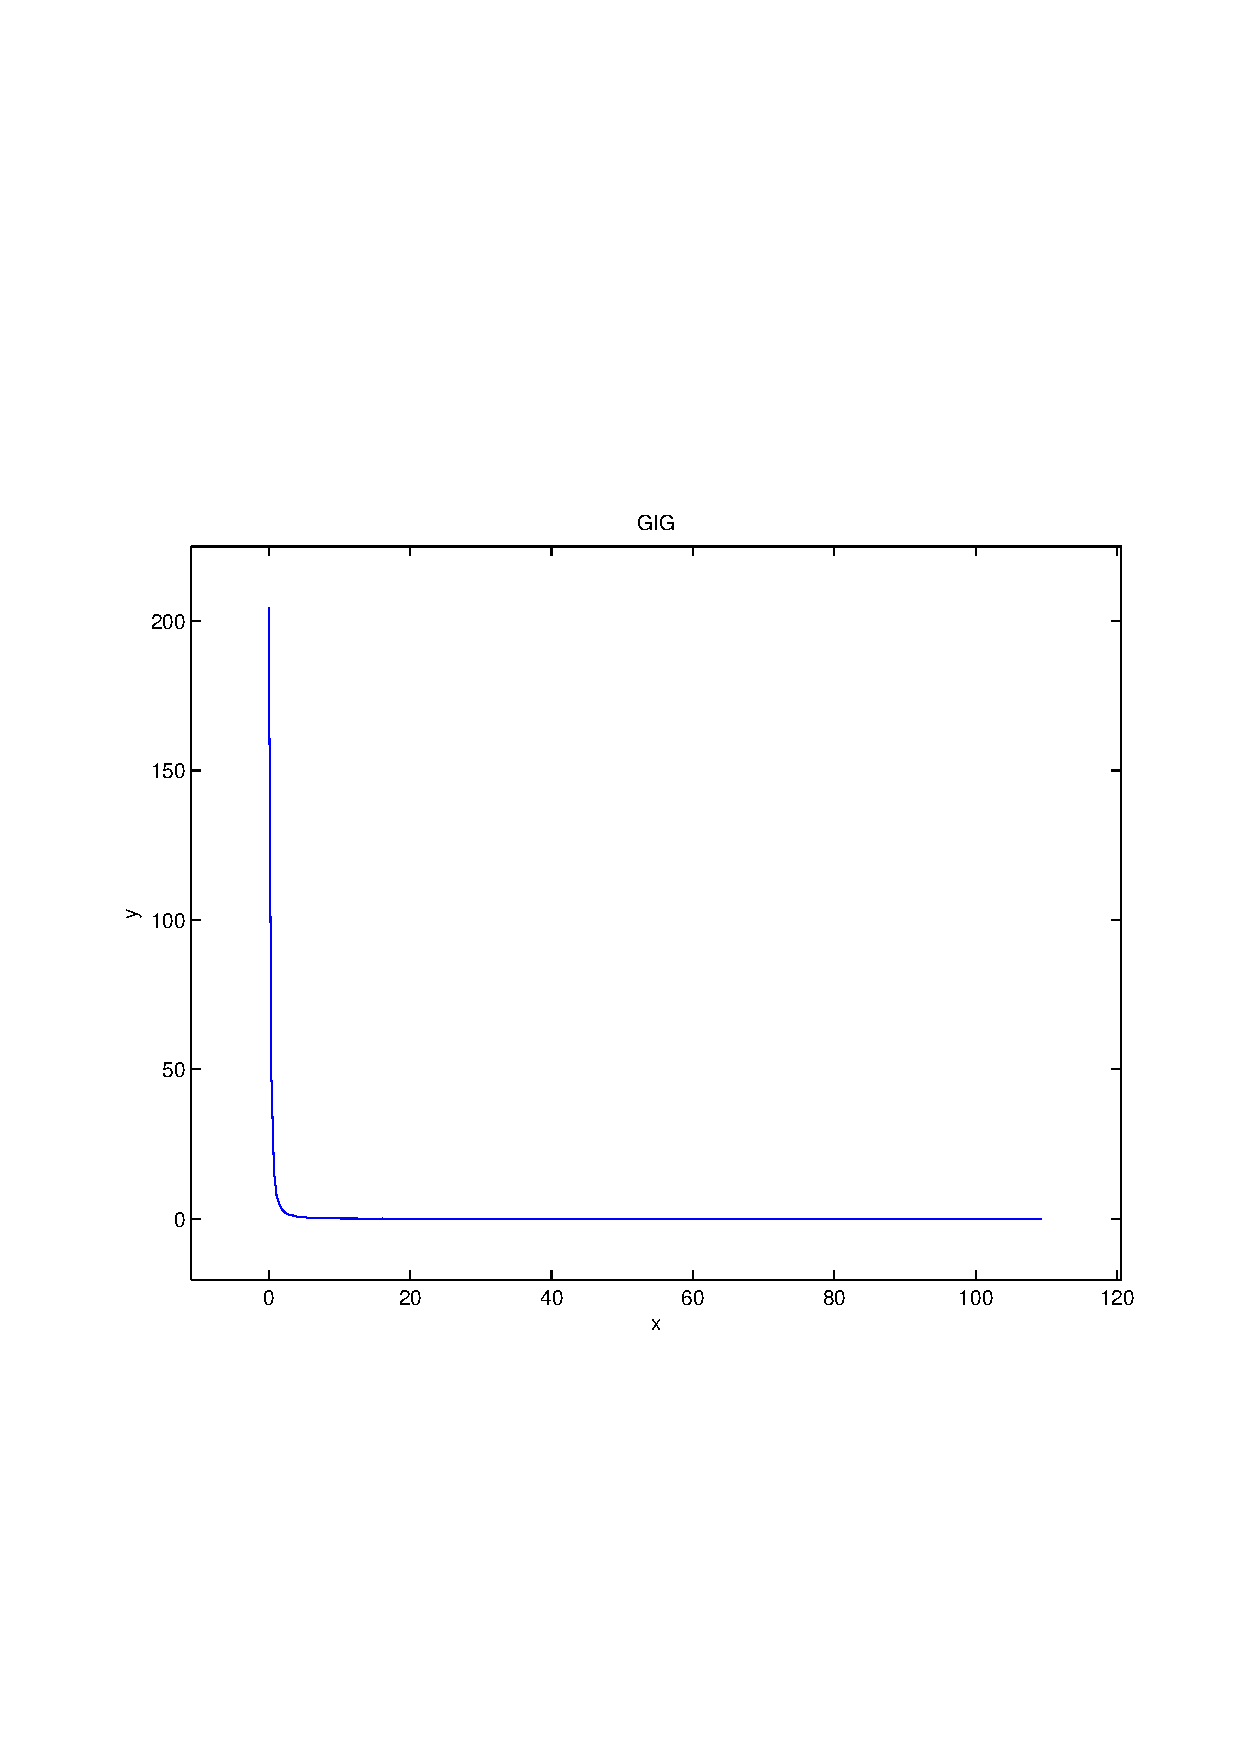
\includegraphics[width=5cm,height=5cm]{GIG.pdf}

normal-box-muller \begin{tabular}{|c|c|c|c|}  mean & variance & skewness & kurtosis \\  \hline
$\mu_1 = -0.001$ & $\mu_2 = +1.002$ & $\mu_3 = -0.003$ & $\mu_4 =+2.966$ \\
\end{tabular}

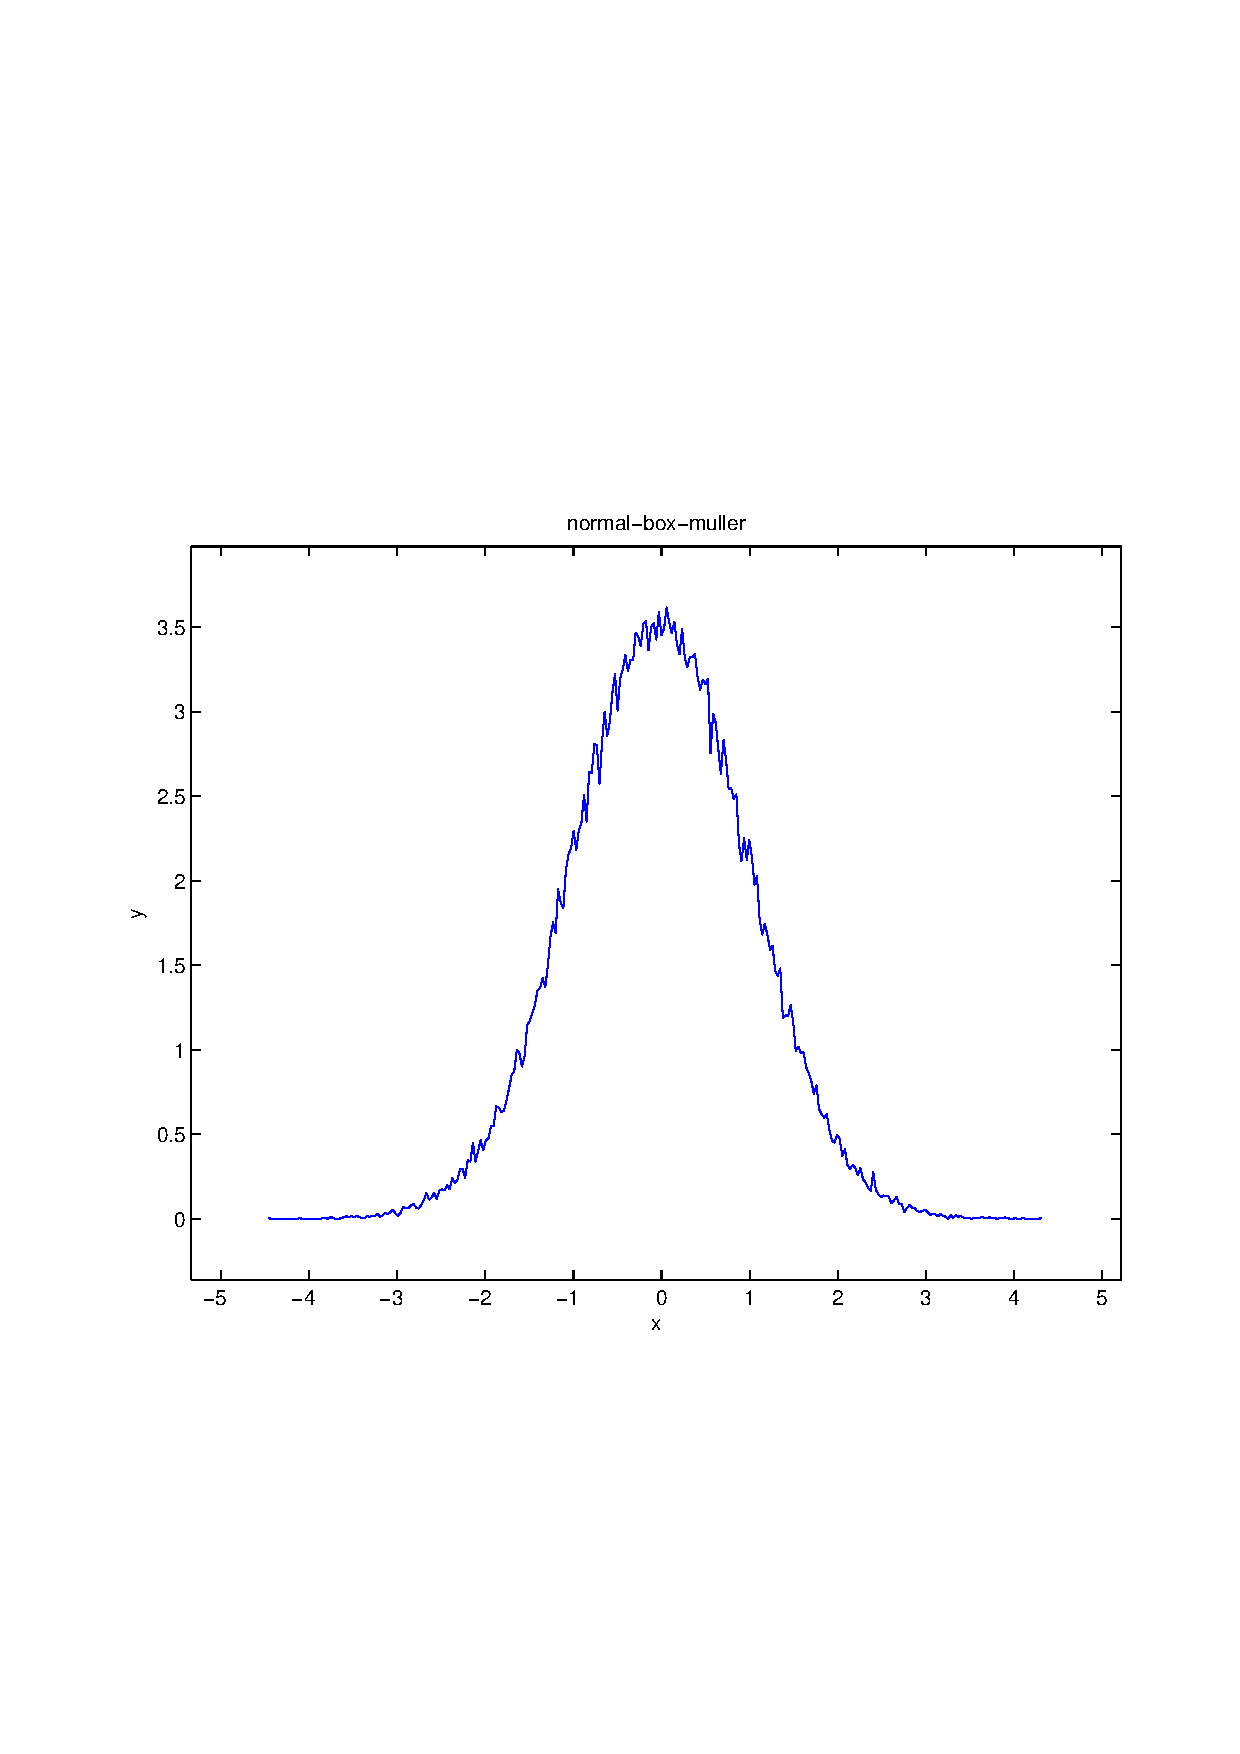
\includegraphics[width=5cm,height=5cm]{normal-box-muller.pdf}

\newpage
normal-inverse-approximation \begin{tabular}{|c|c|c|c|}  mean & variance & skewness & kurtosis \\  \hline
$\mu_1 = +0.002$ & $\mu_2 = +1.005$ & $\mu_3 = +0.012$ & $\mu_4 =+2.993$ \\
\end{tabular}

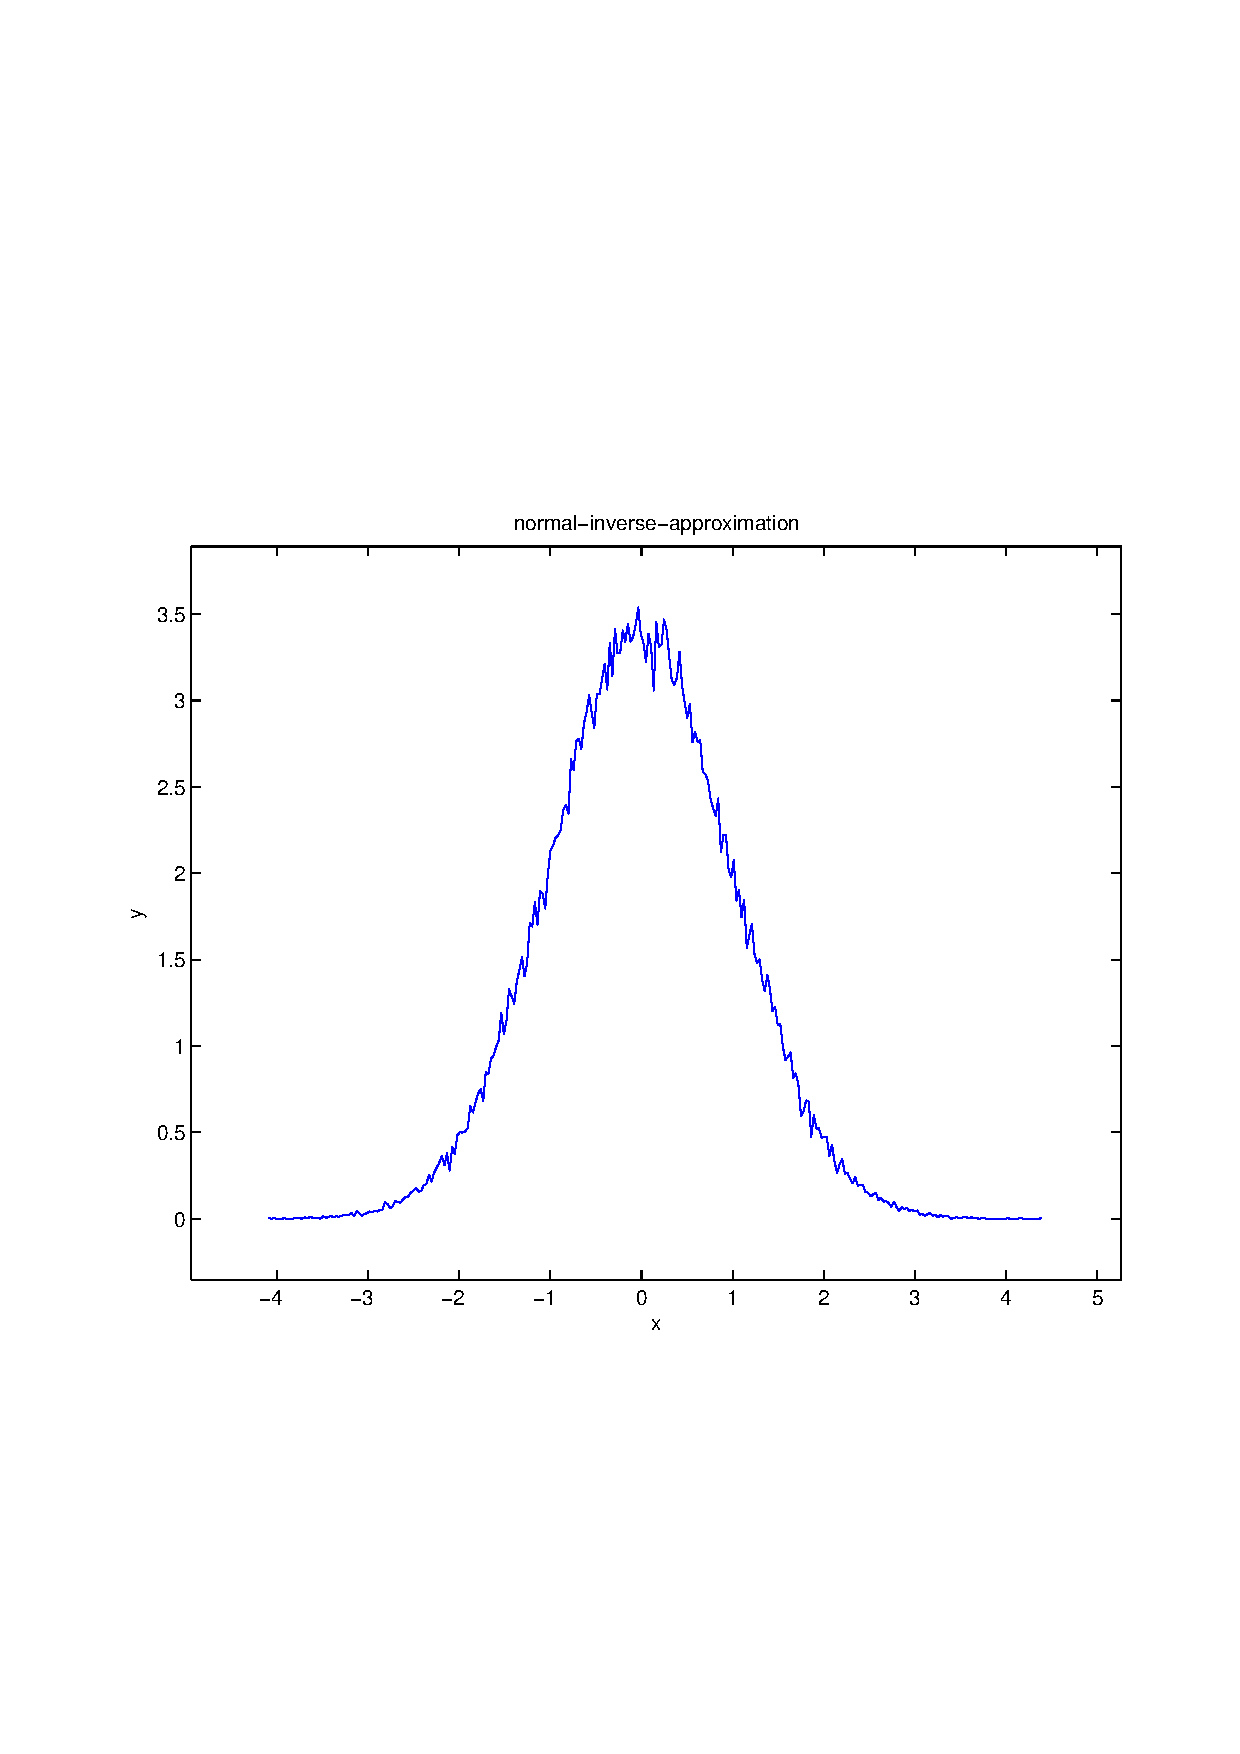
\includegraphics[width=5cm,height=5cm]{normal-inverse-approximation.pdf}

pareto \begin{tabular}{|c|c|c|c|}  mean & variance & skewness & kurtosis \\  \hline
$\mu_1 = +3184578.265$ & $\mu_2 = +888468246174112900.000$ & $\mu_3 = +315.370$ & $\mu_4 =+99629.098$ \\
\end{tabular}

\includegraphics[width=5cm,height=5cm]{pareto.pdf}

poisson \begin{tabular}{|c|c|c|c|}  mean & variance & skewness & kurtosis \\  \hline
$\mu_1 = +1.107$ & $\mu_2 = +0.134$ & $\mu_3 = +3.961$ & $\mu_4 =+21.880$ \\
\end{tabular}

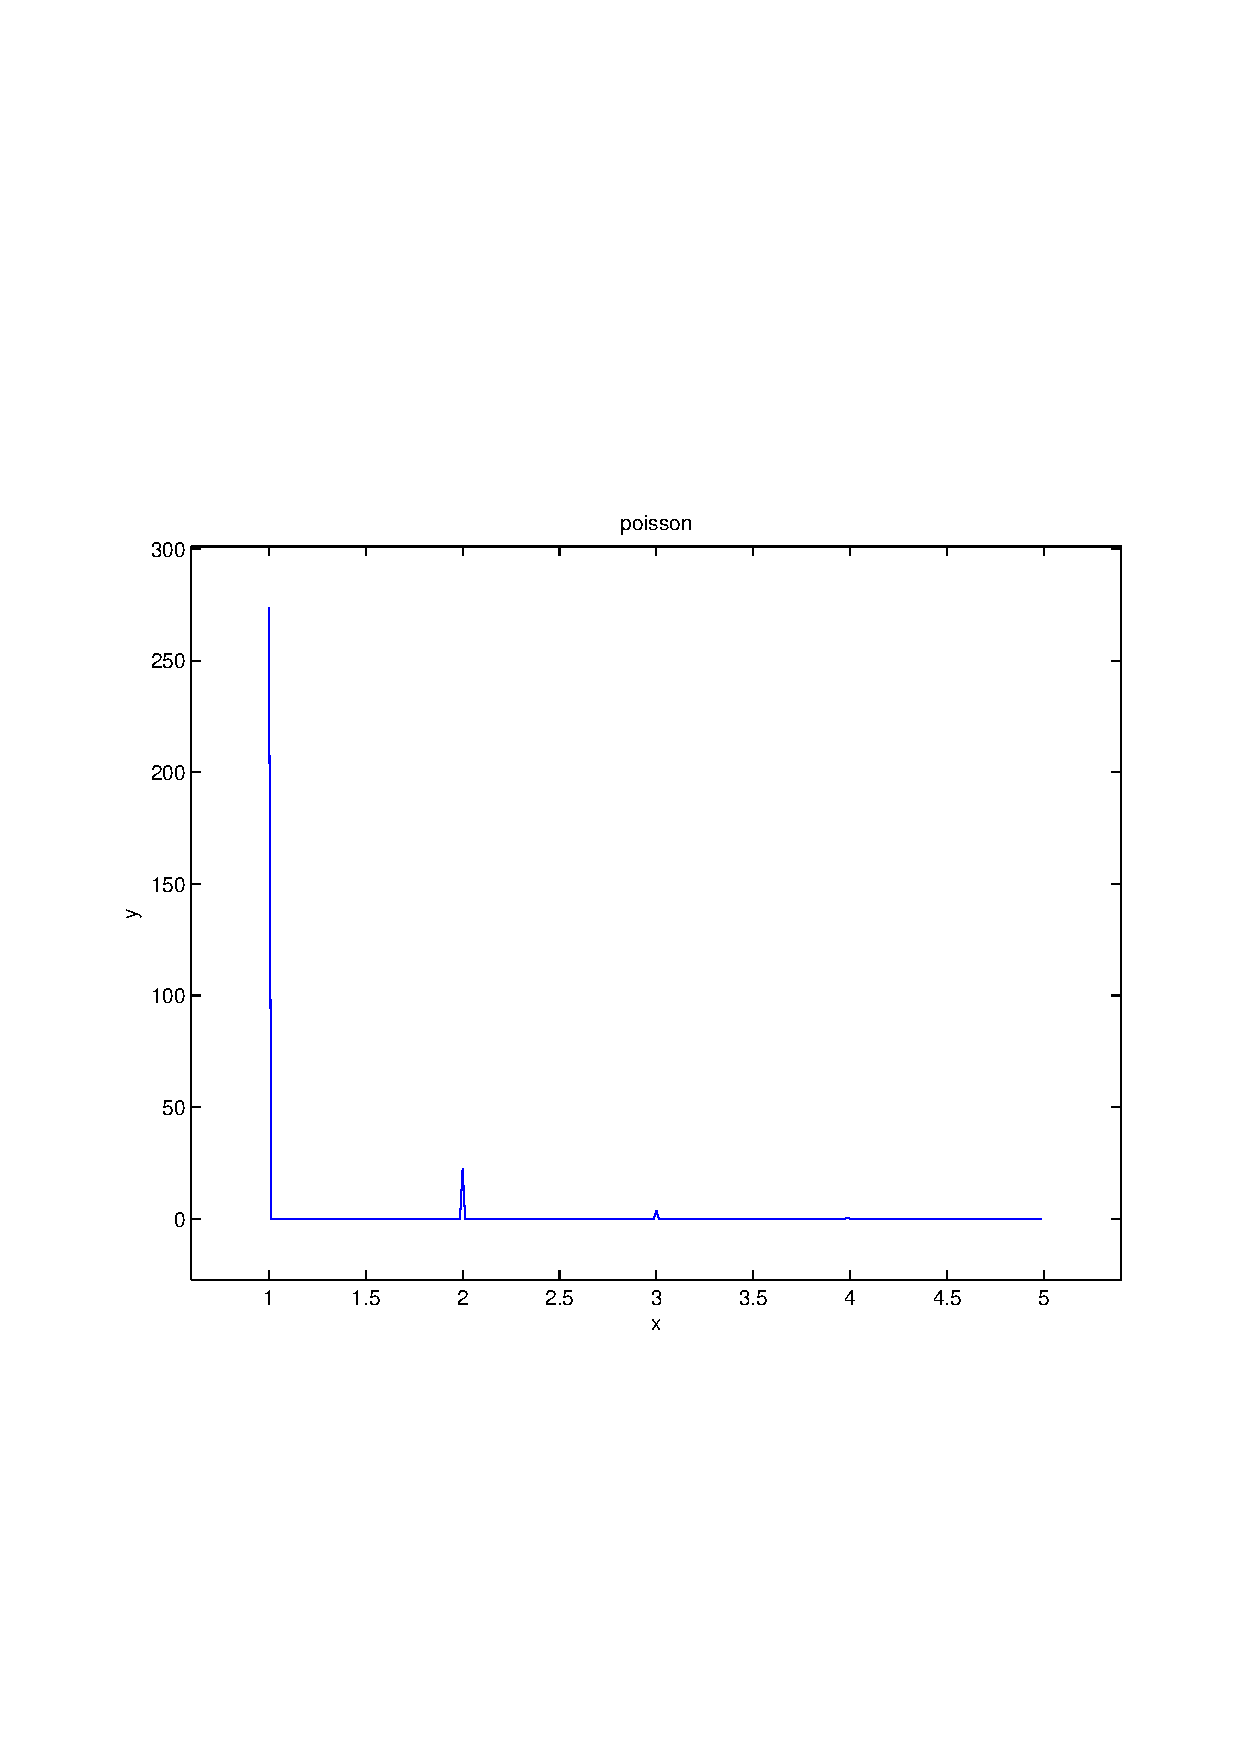
\includegraphics[width=5cm,height=5cm]{poisson.pdf}

\newpage
beta \begin{tabular}{|c|c|c|c|}  mean & variance & skewness & kurtosis \\  \hline
$\mu_1 = +0.335$ & $\mu_2 = +0.127$ & $\mu_3 = +0.672$ & $\mu_4 =+1.899$ \\
\end{tabular}

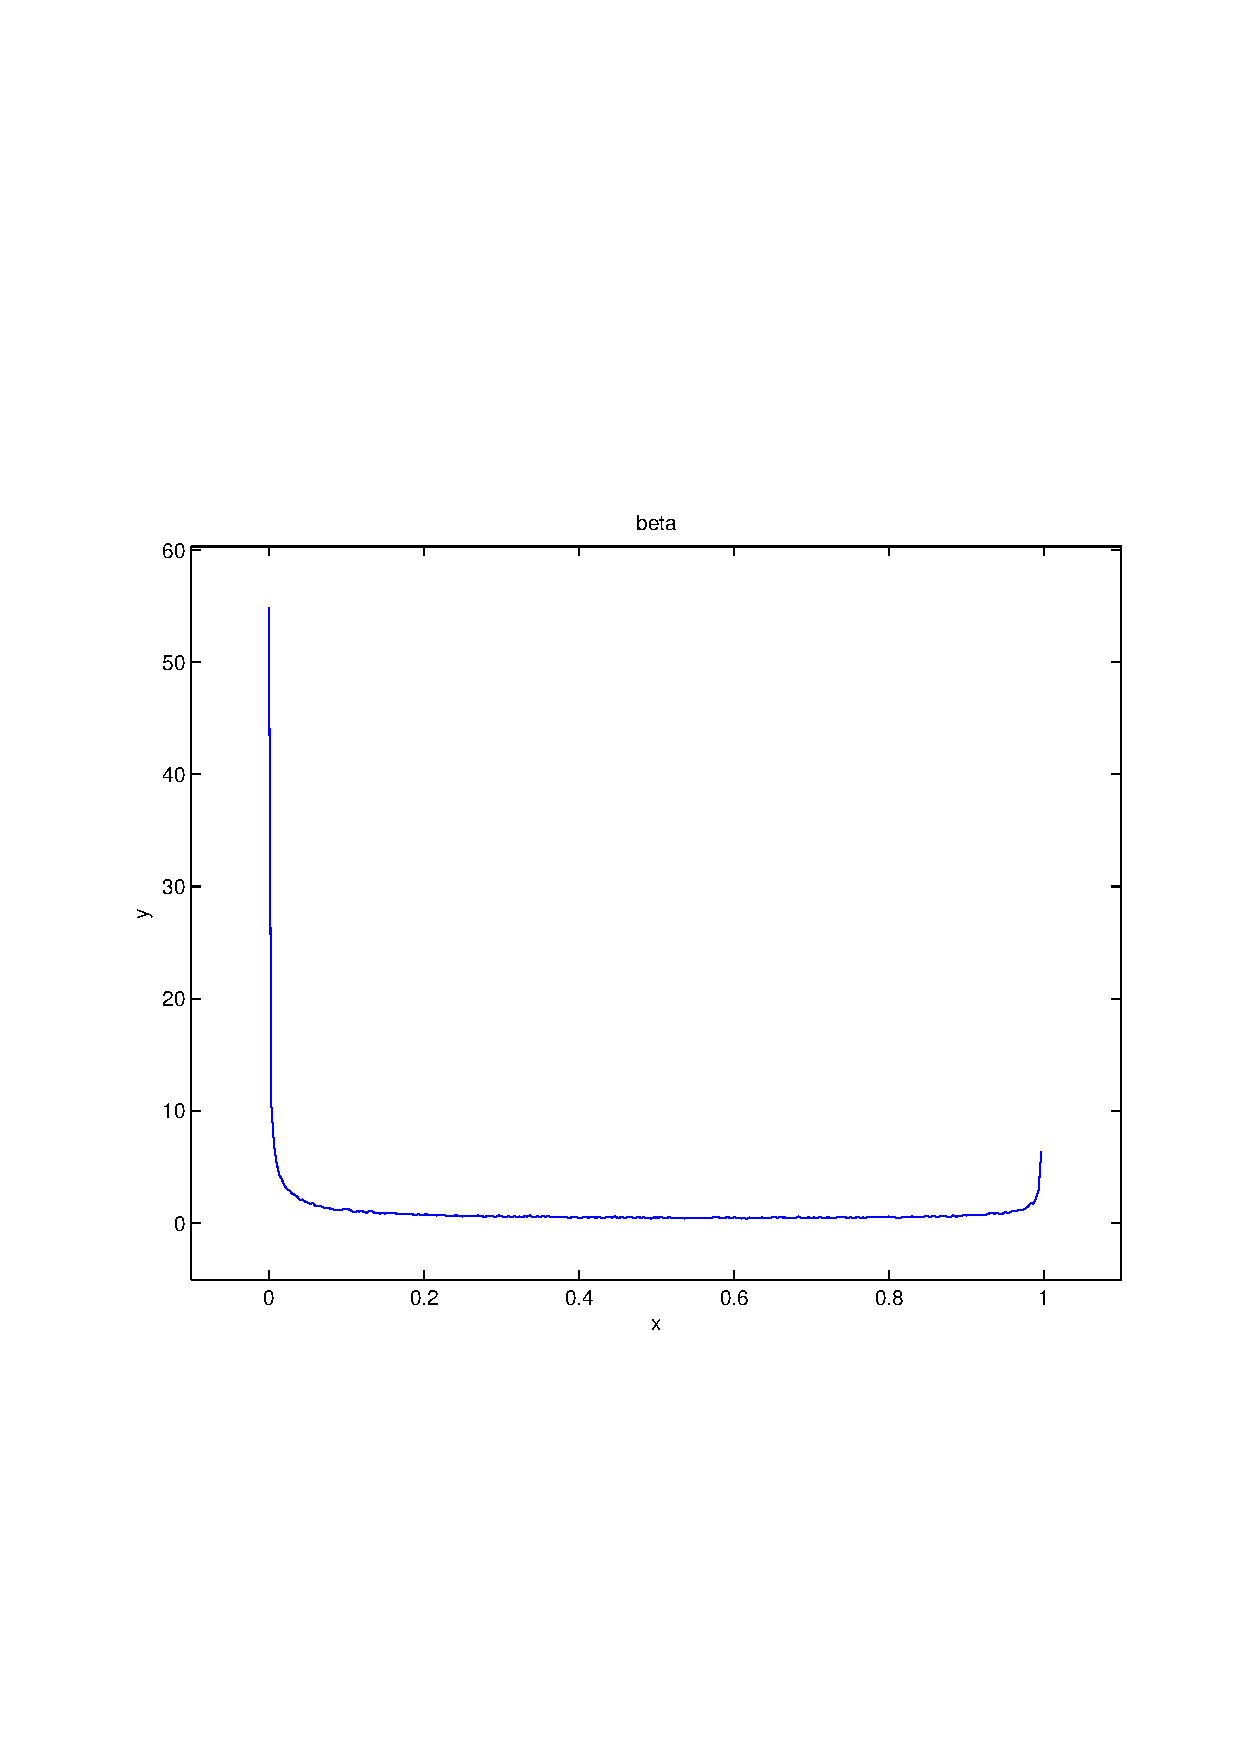
\includegraphics[width=5cm,height=5cm]{beta.pdf}

QueryPerformanceCounter  =  +22.757
\subsubsection{ARPACK}
Running Arnoldi Krylov algorithm on an $n=64$ dimensional $GOE$ matrix.
\subsubsection{Semidefinite Programming SDPA}
QueryPerformanceCounter  =  +0.180
\subsubsection{Linear Regression 3x1}
\subsubsection{3 x 1 Linear Regression}
Sample size = 64

Number of features = 3

$\sigma = \left(
\begin{array}{
ccc}
+3.952 & -0.499 & -0.010 \\
-0.499 & +1.895 & +0.465 \\
-0.010 & +0.465 & +4.477 \\
\end{array}
\right)$

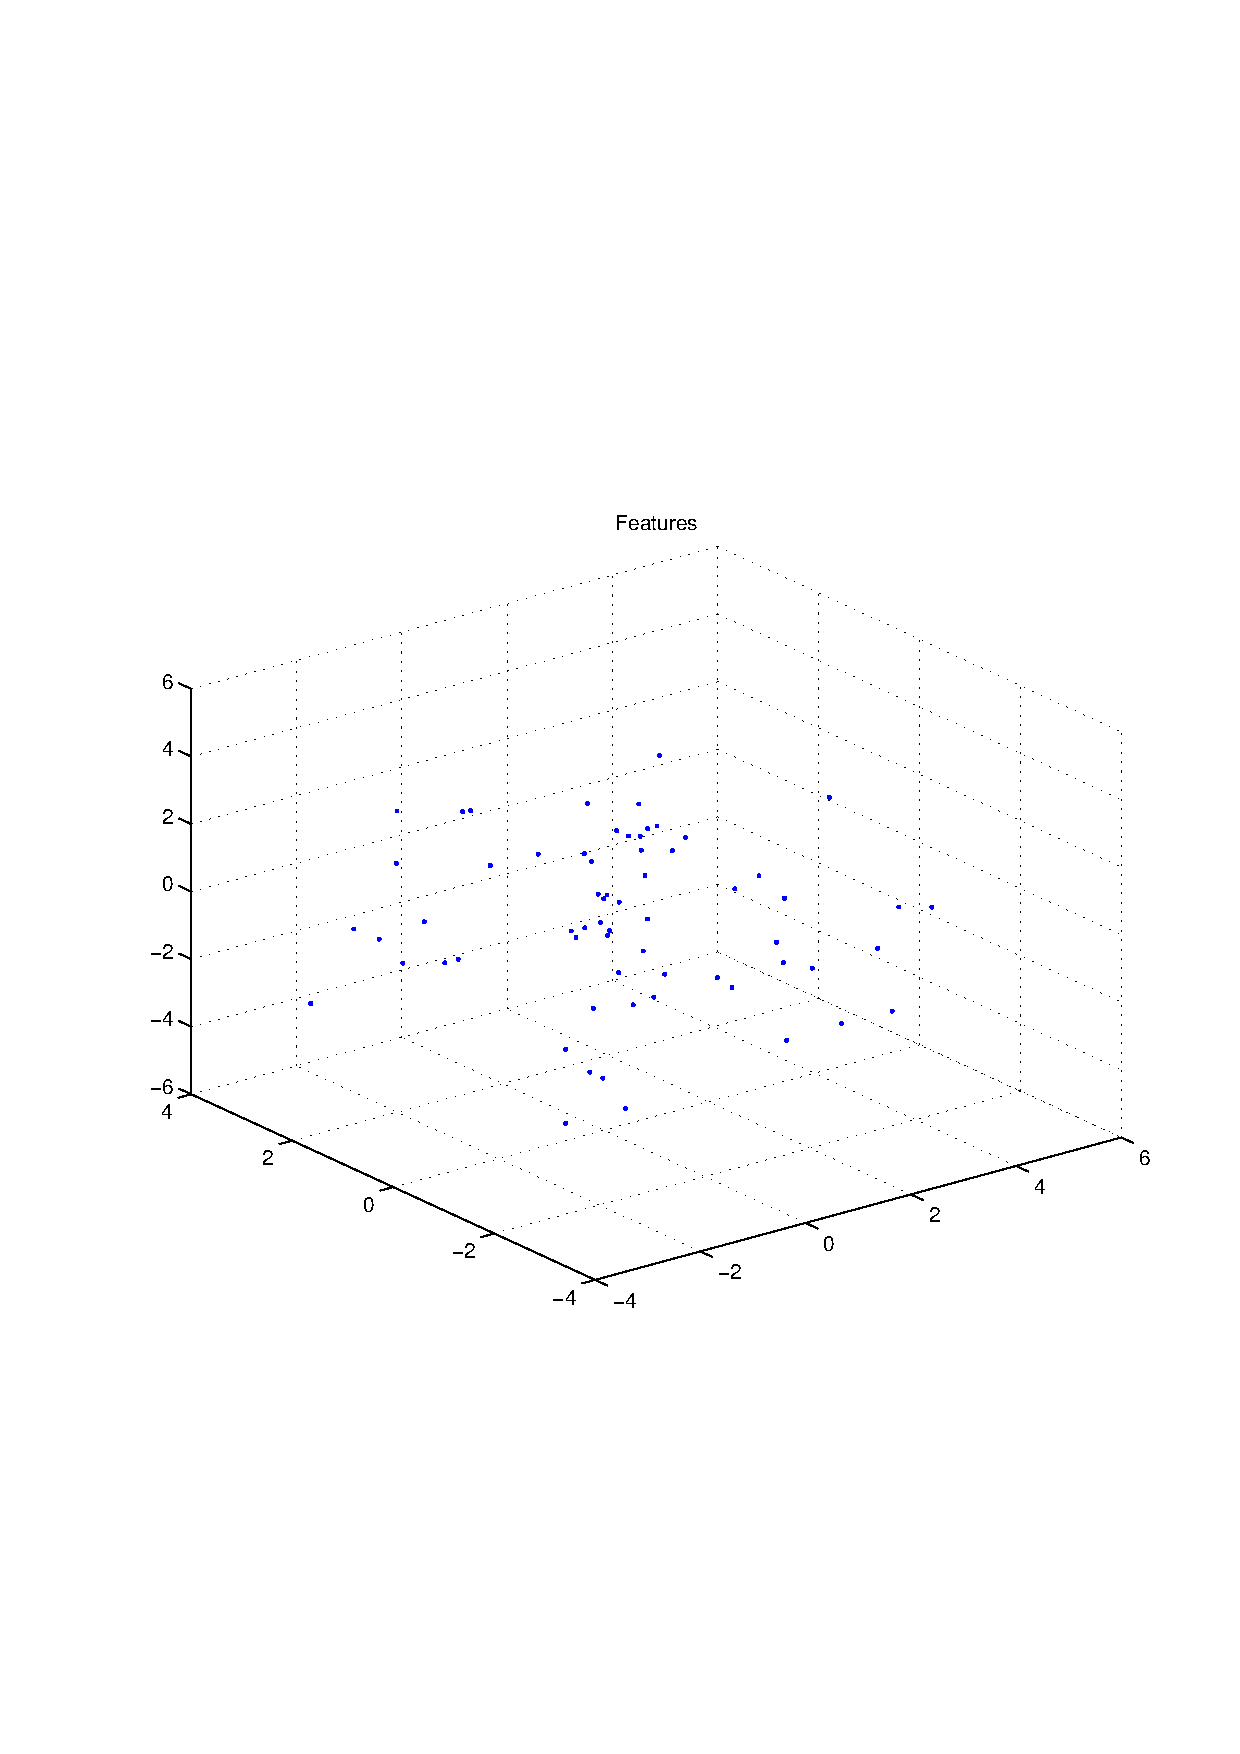
\includegraphics[width=10.0cm,height=10.0cm]{regression_features.pdf}

Beta
+0.817, +0.999, +0.510

Response
-1.476
+2.424
-2.653
+1.621
-0.966
+1.698
+1.904
+5.242
-0.281
+2.553
+3.060
+0.660
-2.792
+0.776
-4.237
+4.428
-0.342
+4.636
+1.416
+3.347
-0.866
+2.712
+0.363
+5.038
-0.152
-2.174
+0.078
-1.179
-0.949
+2.506
+2.557
-0.530
-0.266
+2.899
+2.064
+0.335
-1.821
+2.072
-3.146
+2.893
+1.067
+3.204
-4.721
+0.210
-1.460
-3.465
-0.756
-0.409
+2.859
+1.108
-1.833
+4.569
+2.109
+1.486
-0.630
-2.388
+1.784
-2.650
+0.033
-2.295
+2.529
+0.230
+2.005
+0.811
Estimate for Beta
-6277438562204192200000000000000000000000000000000000000000000000000.000
-6277438562204192200000000000000000000000000000000000000000000000000.000
-6277438562204192200000000000000000000000000000000000000000000000000.000
Error:
-0.000, +0.000, -0.000


QueryPerformanceCounter  =  +1.081
\subsubsection{Matrix Norms}
\subsubsection{Haar Distributed Random Orthogonal Matrix $A \in O(n)$}
 Testing Operator Norm
Number of Dimensions: 3435973836

\subsubsection{Generate Tracey Widom Sample}
\subsubsection{Sample from $W_n m$ times and calculate empirical PDF of the first eig}
This test of the KL libraries will generate histograms of 		  $\lambda_1$ for GOE (Gaussian Orthogonal Ensemble), and W (Wishart) 		  distribution of random matrices

This should approximate the celebrated Tracy Widom distribution.
Dimension $n = 1024$

Sample size $m = 2048$

